\documentclass[12pt,twoside]{article}
\usepackage{amsmath,amsthm,amssymb,amsbsy,epsfig,fancyhdr,calc,ifthen,float,slashbox,psfrag}
\input epsf
\PassOptionsToPackage{ctagsplt,Righttag}{amstex}
\usepackage[dvips,dvipsnames,usenames]{color} % for editing
\usepackage[colorlinks=true,citecolor=MidnightBlue,linkcolor=BrickRed,breaklinks=true]{hyperref}
\usepackage{cite}
\usepackage[boxed,vlined]{algorithm2e}
%-------------- editing ----------------------
\usepackage{color}
\newcommand{\comment}[1]{\textcolor{blue}{[ \sc{#1} ]}} % comments
\newcommand{\revise}[1]{\textcolor{red}{{#1}}} % revisions
%
%******************************MATH DEFINITIONS*********************************
\newcommand{\mb}[1]{{\mbox{\boldmath$#1$\unboldmath}}}
\newcommand{\intd}{\,{\rm d}}
%
%Bold Symbols
%
\newcommand{\beps}{\boldsymbol{\epsilon}}
\newcommand{\bveps}{\boldsymbol{\varepsilon}}
\newcommand{\blambda}{\boldsymbol{\lambda}}
\newcommand{\bxi}{\boldsymbol{\xi}}
\newcommand{\bpi}{\boldsymbol{\pi}}
\newcommand{\bsigma}{\boldsymbol{\sigma}}
\newcommand{\bchi}{\boldsymbol{\chi}}
\newcommand{\bGamma}{\boldsymbol{\Gamma}}
\newcommand{\bPi}{\boldsymbol{\Pi}}
\newcommand{\bXi}{\boldsymbol{\Xi}}
\newcommand{\bLambda}{\boldsymbol{\Lambda}}
%
%Bold Alphabeticals
%
\newcommand{\bA}{\mathbf{A}}
\newcommand{\bB}{\mathbf{B}}
\newcommand{\bC}{\mathbf{C}}
\newcommand{\bD}{\mathbf{D}}
\newcommand{\bE}{\mathbf{E}}
\newcommand{\bF}{\mathbf{F}}
\newcommand{\bG}{\mathbf{G}}
\newcommand{\bH}{\mathbf{H}}
\newcommand{\bI}{\mathbf{I}}
\newcommand{\bJ}{\mathbf{J}}
\newcommand{\bK}{\mathbf{K}}
\newcommand{\bL}{\mathbf{L}}
\newcommand{\bN}{\mathbf{N}}
\newcommand{\bP}{\mathbf{P}}
\newcommand{\bQ}{\mathbf{Q}}
\newcommand{\bR}{\mathbf{R}}
\newcommand{\bS}{\mathbf{S}}
\newcommand{\bT}{\mathbf{T}}
\newcommand{\bU}{\mathbf{U}}
\newcommand{\bX}{\mathbf{X}}
\newcommand{\bY}{\mathbf{Y}}
\newcommand{\ba}{\mathbf{a}}
\newcommand{\bb}{\mathbf{b}}
\newcommand{\bc}{\mathbf{c}}
\newcommand{\bd}{\mathbf{d}}
\newcommand{\be}{\mathbf{e}}
\newcommand{\ff}{\mathbf{f}}
\newcommand{\bg}{\mathbf{g}}
\newcommand{\bh}{\mathbf{h}}
\newcommand{\bl}{\mathbf{l}}
\newcommand{\bm}{\mathbf{m}}
\newcommand{\bn}{\mathbf{n}}
\newcommand{\bp}{\mathbf{p}}
\newcommand{\bq}{\mathbf{q}}
\newcommand{\br}{\mathbf{r}}
\newcommand{\bt}{\mathbf{t}}
\newcommand{\bu}{\mathbf{u}}
\newcommand{\bv}{\mathbf{v}}
\newcommand{\bw}{\mathbf{w}}
\newcommand{\bx}{\mathbf{x}}
\newcommand{\by}{\mathbf{y}}
\newcommand{\mC}{\mathbb C}
%
% Caligraphics
%
\newcommand{\cA}{\mathcal{A}}
\newcommand{\cC}{\mathcal{C}}
\newcommand{\cD}{\mathcal{D}}
\newcommand{\cE}{\mathcal{E}}
\newcommand{\cF}{\mathcal{F}}
\newcommand{\cH}{\mathcal{H}}
\newcommand{\cI}{\mathcal{I}}
\newcommand{\cJ}{\mathcal{J}}
\newcommand{\cK}{\mathcal{K}}
\newcommand{\cL}{\mathcal{L}}
\newcommand{\cN}{\mathcal{N}}
\newcommand{\cP}{\mathcal{P}}
\newcommand{\cQ}{\mathcal{Q}}
\newcommand{\cU}{\mathcal{U}}
\newcommand{\cV}{\mathcal{V}}
\newcommand{\cX}{\mathcal{X}}
%
% Fraktur
%
\newcommand{\fI}{\mathfrak{I}}
\newcommand{\fK}{\mathfrak{K}}
\newcommand{\fL}{\mathfrak{L}}
%
% Bold numbers
%
\newcommand{\bzero}{\boldsymbol{0}}
%
% Operator names
%
\newcommand{\argm}{\operatorname{arg}}
\newcommand{\argmin}{\operatorname{argmin}}
\newcommand{\Div}{\operatorname{Div}}
\newcommand{\Grad}{\operatorname{Grad}}
\newcommand{\norm}[1]{\left|\left|#1\right|\right|} 
%
%********************************** TIME PRINT**********************************
%
\newcounter{hours}
\newcounter{minutes}
\newcommand{\printtime}{\setcounter{hours}{\time/60}%
                        \setcounter{minutes}{\time-\value{hours}*60}%
\ifthenelse{\value{hours}<10}{0}{}\thehours:%
\ifthenelse{\value{minutes}<10}{0}{}\theminutes}
%
%**********************AMENDMENTS TO FANCYHDR STYLE*****************************
%
\renewcommand{\headrulewidth}{0.8pt}
%\renewcommand{\footrulewidth}{0.8pt}
\fancyhf{}
\fancyhead[RE]{\sl \thepage}
\fancyhead[RO]{\rm \thepage}
%\fancyfoot[CE,CO]{\rm \thepage}
%
% *****************************SIZE DECLARATIONS*******************************
%
\def\lsp{\def\baselinestretch{0.75}\large\normalsize}
\def\ssp{\def\baselinestretch{1.0}\large\normalsize}
\def\dsp{\def\baselinestretch{1.37}\large\normalsize}
\oddsidemargin 19pt \evensidemargin 19pt \marginparwidth 100pt
\marginparwidth 0.5in
\marginparsep 10pt
\topmargin -30pt
\headheight 20pt \headsep 25pt \footskip 35pt
\textheight = 615pt
\advance\textheight by \topskip
\textwidth 430pt \columnsep 10pt \columnseprule 0pt
\parskip 0pt plus 1pt
\parindent 17pt
\partopsep 3pt plus 1pt minus 2pt
%\footnotesep 2pt
%
% *****************************DEFINITIONS**************************************
%
\newcommand{\figref}[1]{Figure \ref{#1}}
\makeatletter
\newenvironment{tablehere}
  {\def\@captype{table}}
  {}
\newenvironment{figurehere}
  {\def\@captype{figure}}
  {}
\makeatother
%
%*******************************DOCUMENT BEGIN**********************************
%
\begin{document}
\bibliographystyle{unsrt}
\flushbottom
\pagestyle{empty}
\pagenumbering{arabic}
%**********************************TITLE PAGE***********************************
%
\ssp


\begin{titlepage}

\begin{center}
{\Huge A Simple Cartesian Grid Finite Element Method Using Cut Cells}\\
 \vspace{0.5cm}
by\\
 \vspace{0.5cm}
Meriem Ben-Salah\\
 \vspace{0.5cm}
MS (Leibniz University of Hanover) 2008\\ 
 \vspace{1.5cm} 
A report submitted in partial satisfaction of the\\ 
 \vspace{0.5cm}
Requirements for the degree of\\  
 \vspace{0.5cm} 
Masters of Science, Plan II\\  
 \vspace{0.5cm} 
in\\  
 \vspace{0.5cm} 
Mechanical Engineering\\  
 \vspace{0.5cm} 
at the\\  
 \vspace{0.5cm}
University of California at Berkeley\\  
  \vspace{1.5cm}
Committee in Charge: \\ 
 \vspace{0.5cm}
 \begin{center}
\line(1,0){250}
\end{center}
Professor Panayiotis Papadopoulos, Chairman\\  
 \vspace{1.0cm}
 \begin{center}
\line(1,0){150}
\end{center}
Professor Phillip Colella\\  
  \vspace{1.5cm}
Fall 2011\\  
\end{center}




\end{titlepage}

%\title{\vspace{-0.75in}\bf  A Simple Cartesian Grid Finite Element Method Using Cut Cells \rm}
%\vspace{0.1in}
%\author{\hspace{-0.65in}Meriem BEN SALAH\thanks{Department of Mechanical Engineering, University of California, Berkeley}, Panayiotis PAPADOPOULOS\thanks{Department of Mechanical Engineering, University of California, Berkeley, corresponding author}}
%\date{}
%\maketitle
\begin{center}
{\textbf{Abstract}}
\end{center}
The cost and quality of unstructured Finite Element meshes have been and still are a stumbling block of the Finite Element Analysis. While the effect and cost of the unstructured mesh quality on the numerical convergence are improved, research is being conducted on developing new methodologies using the simplest mesh possible, a rectangular grid. In this master's report, a novel method for solving two-dimensional partial differential equations, using the Finite Element method on a uniform linear rectangular grid that is non-fitted to the domain boundary is presented. An algorithm for obtaining maximal accuracy from regular grids with minimal boundary intervention is presented. A new approach for applying Dirichlet and Neumann boundary conditions using the partial cells nodal information is developed in one-dimension and in two-dimensions. The partial cells method preserves the convergence order obtained by Finite Element solutions using unstructured meshes for the Dirichlet type of boundary conditions.  For some set of problems, the method performs even better than the classical Finite Element method due to the quality of the rectangular grid elements.  An adequate trade-off between accuracy and computational performance is experienced.  A slight loss of sparsity and a numerically tolerable increase in the condition number of the Finite Element system arise. The accuracy of the partial cells Finite Element method is shown to be negligibly sensitive to the location of the physical domain with respect to the rectangular grid. 
\begin{description}
\item[Keywords:] Finite Element, Cartesian Grid, Cut Cell
\end{description}
%
%******************************ACKNOWLEDGMENTS**********************************
%
\protect\vspace{0.2in}
\begin{center}
{\textbf{Acknowledgments}}
\end{center}
Research supported by Microsoft (Award \#024263 ) and Intel (Award \#024894) funding and by matching funding by U.C. Discovery (Award \#DIG07-10227).
\newpage
%\renewcommand{\contentsname}{\normalsize\centerline{Table of contents}}
%\vspace{-0.25in}
\tableofcontents
\ssp
\protect\vspace{0.25in}
\normalsize
\protect\vspace{0.1in}
\nopagebreak[4]
\dsp
\newpage
\listoffigures
\newpage
\listoftables
\newpage
\pagestyle{fancyplain}
%*******************************************************************************
\section{Introduction}\label{sec:intro}
%\begin{itemize}
%\item State of art from elements and volumes (related work)
%Boeing cut-cells phantom methods (ocean) 
\par The cost and quality of unstructured Finite Element meshes have been and still are a stumbling block of the Finite Element Analysis. While the effect and cost of the unstructured mesh quality on the numerical convergence are improved, research is being conducted on developing new methodologies using the simplest mesh possible, a rectangular grid. The latter set of methods are appealing because of their meshing and mathematical simplicity. Moreover, mesh adaptivity, the use of multigrid solvers and coupling to physical submodeling are easily adoptable.  When modeling fluid dynamics in irregular geometries, Colella (\cite{colella2}, \cite{colella})  uses an embedded boundary volume-of-fluid method, where the intersection of each grid cell with the free boundary, a cut-cell, is specified. The dependent variables are approximated at the centers of the rectangular grid volumes. Johnson (\cite{tranair}, \cite{tranair2}, \cite{tranair3}) presents the Boeing TRANAIR rectangular grid finite element method, where the boundary surfaces are prescribed via a network of panels.  Recursion is necessary for accurate panel locations. Venkatasubban determines with the Bombardier-Learjet EULAIR method (\cite{eulair}, \cite{eulair2}) the cut-cell region of a rectangular grid by solely the knowledge of integration points on the boundary. Recursion is not necessary in this case. The NASA TIGER solver developed by Melton et. al. (\cite{tiger}, \cite{tiger2}, \cite{tiger3}, \cite{tiger4}) is a Finite Volume Method that uses non-body-fitted cartesian grids and a border of irregularly shaped  cells at the intersection between the grid and the geometry.  Young et. al. \cite{young} handle boundary regions through adaptive refining in the proximity of the domain boundary.  
%\item %Statement of the problem
%Try to obtain maximal accuracy from regular grids with minimal boundary intervention
\par In this master's report, a novel method for solving two-dimensional partial differential equations using the Finite Element method on a uniform linear rectangular grid that is non-fitted to the domain boundary is presented. An algorithm for obtaining maximal accuracy from regular grids with minimal boundary intervention is presented. The rectangular grid elements containing arbitrarily shaped domain boundaries are christened partial elements. A new approach for applying Dirichlet and Neumann boundary conditions using the nodal information of the partial cells is developed. The method preserves the convergence order obtained by Finite Element solutions using unstructured meshes for the Dirichlet type of boundary conditions.  For some set of problems, the method performs even better than the classical Finite Element method due to the quality of the rectangular grid elements.  An adequate trade-off between accuracy and computational performance is experienced.  A slight loss of sparsity and a numerically tolerable increase in the condition number of the Finite Element system arise. The accuracy of the partial cells Finite Element method is shown to be negligibly sensitive to the location of the physical domain with respect to the rectangular grid. 
%\item Our methodology (novel aspects)
%Based on cut cells 
\par The partial cells method supplements the Finite Element method with the use of rectangular grid without the need for adaptive or conforming meshing along the boundary. Partial elements that are traversed by the domain boundary are distinguished from regular elements that are fully contained in the domain, full elements. Full elements are treated in the classical manner. The treatment of partial elements  leads to the fulfillment of boundary conditions. Nodes of the partial grid that lie outside the domain, which are called hanging nodes, do not contribute to the interpolation of the partial differential equation. Involving the degrees of freedom associated with all nodes of the partial element, linear collocation equations are calculated based on the location of the portion of the boundary contained in the partial element. Thereafter, the equations are assigned to the hanging degrees of freedom and assembled in the global system. 
%\item Organization of paper
\par First, the partial cells method in one-dimension is presented and convergence in the H$^0$ and  H$^1$ error norms is shown in Section \ref{sec:oned}. The effect of the size of the partial domain on the convergence of the method is studied. In Section \ref{sec:attempted}, methods  that were attempted and compared for preliminary evaluations of the partial cells method are presented. In Section \ref{sec:twod},  the method is presented in a two-dimensional setting. The convergence behavior for several boundary value problems is studied. The effect of randomness of the location of the domain boundary with respect to the rectangular grid is studied. In addition, the numerical performance of the partial cells method is compared to classical Finite element methods using unstructured meshes.  In Section \ref{sec:conc}, the report is concluded with some remarks and future work. 
%\end{itemize}
%*******************************************************************************
\newpage
\section{Motivation from One-Dimension}\label{sec:oned}
\par
In this section, the proposed method is motivated from a simple one-dimensional 
problem, which illustrates most of the salient features and the derived 
response to various approaches for dealing with irregular boundaries. 
%-------------------------------------------------------------------------------
\subsection{Method}\label{sec:methods1d}
\par
Consider a scalar second-order differential equation on a one-dimensional 
domain $(0,1)$ that is to be solved by a Galerkin method-based finite element 
approximation. Let a spatially uniform discretization of the domain with size 
$h=1/n$ be constructed, such that the left boundary point ($x=0$) is occupied 
by the first finite element node, while the right boundary point 
($x=1$) does not coincide with a node. Thus, the last element is only partially 
occupying the physical domain of the problem, as in Figure~\ref{fig:onedomain}. 
To solve the differential equation by the finite element method using this 
regular mesh, one may proceed to: 
\begin{enumerate}
\item Compute the element arrays for all elements including the last element. 
\item After assembly, eliminate the equation associated with the degree 
of freedom of the node that lies outside the physical domain. 
\item Substitute the eliminated equation by an interpolation equation to 
impose the boundary condition at $x=1$. 
\end{enumerate}
Regardless of the type of domain element used for the solution, there are 
several possible interpolation choices for the partial element. Assuming that 
the physical domain covers a region of size $\alpha h$ 
($0<\alpha<1$) inside the rightmost subdomain $(x_n,x_{n+1})$ 
in Figure~\ref{fig:onedomain}, these include: 
\begin{itemize}
%
\item[a.] Linear interpolation: Imposing a Dirichlet boundary condition, 
$u\vert_{x=1} = \overline{u}$, one readily finds the interpolation
equation 
%
\begin{equation}\label{eq:linD}
\overline{u}\ =\ N_n(\alpha h)u_{n}+N_{n+1}(\alpha h)u_{n+1}\ ,
\end{equation}
%
where $N_n(t) = -\frac{(t-h)}{h}$ and 
$N_{n+1}(t)= \frac{t}{h}$. Alternatively, to impose the associated Neumann boundary condition 
$\frac{\text{d}u}{\text{d}x}\vert_{x=1} = \overline{q}$, one finds that 
%
\begin{equation}\label{eq:linN}
\overline{q}\ =\ 
\frac{\text{d}N_n}{\text{d}x}(\alpha h)u_n+
\frac{\text{d}N_{n+1}}{\text{d}x}(\alpha h)u_{n+1}\ .
\end{equation}
Either equation \eqref{eq:linD} or \eqref{eq:linN} would be used in lieu of the 
eliminated equation associated with the degree of freedom of node $n+1$. 
%
\item[b.] Quadratic Interpolation: It is easy to impose the Dirichlet or
Neumann boundary condition using a quadratic interpolation defined by the 
degrees of freedom of nodes $n-1$, $n$ and $n+1$. For the Dirichlet boundary 
condition case, this leads to 
%
\begin{equation}\label{eq:quadD}
\overline{u}\ =\ N_{n-1}(\alpha h) u_{n-1}+
N_n(\alpha h) u_n + N_{n+1}(\alpha h) u_{n+1}\ , 
\end{equation}
%
where $N_{n-1}(t)= \frac{(t-h)(t-2h)}{2h^2}$, 
$N_{n-1}(t)= -\frac{t(t-2h)}{h^2}$, and 
$N_{n+1}(t)= \frac{t(t-h)}{2h^2}$. We may similarly impose the associated Neumann boundary conditions as 
%
\begin{equation}\label{eq:quadN}
\overline{q}\ =\ 
\frac{\text{d}N_{n-1}}{\text{d}x}(\alpha h)u_{n-1}+
\frac{\text{d}N_{n}}{\text{d}x}(\alpha h)u_{n}+
\frac{\text{d}N_{n+1}}{\text{d}x}(\alpha h)u_{n+1}\ .
\end{equation}
%
\end{itemize}
Figure \ref{fig:linear} shows the two kinds of interpolation. Higher-order interpolations are also possible, but will not be discussed here. 
%-------------------------------------------------------------------------------
\subsection{Convergence analysis}\label{sec:convergence1d}
\par
The preceding methods are analyzed using a simple test problem to appreciate 
the rates of convergence attained by the interpolation of the boundary 
condition at $x=1$. The test problem is specified as follows: 
%
\begin{eqnarray}
\frac{\text{d}^2 u}{\text{d} x^2} &=& -x \hspace{0.5cm}\text{on}\hspace{0.5cm}0 < x < 1,\\
u\vert_{x=0} &=& 0 . 
\end{eqnarray}
%
The Dirichlet boundary condition is set to 
%
\begin{equation}\label{eq:D1}
\overline{u}\ =\ 0.5\ \quad \text{at } x=1\ ,
\end{equation}
%
while, alternatively, the corresponding Neumann boundary condition is 
%
\begin{equation}\label{eq:N1}
\overline{q}\ =\ 0.5 \quad \text{at } x=1\ . 
\end{equation}
%
In addition, the parameter $\alpha$ is set to $\alpha=0.5$, which means that 
the physical boundary bisects the last subdomain 
$(x_n,x_{n+1})$.  
%
\subsubsection{Dirichlet-Dirichlet Model Problem}
\par
In the Dirichlet-Dirichlet case, where the boundary condition~\eqref{eq:D1} 
is enforced, the interpolation of the dependent variable is taken to
be quadratic over the last two elements. 
Figure~\ref{fig:femdirichlet1dH0} shows the rates of convergence in the H$^0$ and $H^1$ norm,
respectively. The rates of convergence are 2 and 1, hence are identical to 
those expected of conventional elements without any special treatment related 
to partial cells, see, e.g., \cite{CIARLET80}. \\
\subsubsection{Dirichlet-Neumann Model Problem}
\par
The theoretical rates are also observed in the case of the
Dirichlet-Neumann problem, which makes use of the boundary
condition~\eqref{eq:N1}. Here, the interpolation of the flux 
results from taking the derivative of the (quadratic) interpolation of
the dependent variable over the last two elements of the domain. 
The relevant results for the H$^0$ and H$^1$ norm are shown 
in Figure~\ref{fig:femneumann1dH0}. 
\subsubsection{Partial Element Effect on Convergence}
\par
For the preceding one-dimensional problem, the finite element method 
exhibits the same order of convergence independently of the type 
of boundary conditions imposed. It is important to investigate whether
these rates persist independently of the size of the partial element
containing the boundary of the domain and that the recovered results
are, hopefully, insensitive to the specific placement of the actual
boundary point in the last element of the mesh. Therefore, the
previous canonical problem is resolved by varying the location of the
boundary of the physical domain with respect to the finite element mesh. 
\par
By varying the size of the (uniform) mesh, three different partial coverings of
the last domain element by the physical domain are defined: they cover 
the leftmost $30\%$ ($0.3$), $50\%$ ($0.5$) of $80\%$ ($0.8$) of the
last element's domain. The convergence rates in the H$^0$ and H$^1$ norms 
for the Dirichlet-Dirichlet boundary problem are shown 
in Figure \ref{fig:dirichlet1dh0alpha030508}. For all three cases,
the same rates apply, which shows that there is no sensitivity to the
size of the partial element. \\
The rates of convergence for the Dirichlet-Neumann problem exhibit the
same insensitivity to the size of the partial element, provided that
a linear interpolation of the flux is effected, as described earlier
in this section. Figure~\ref{fig:neumann1dlinearh0alpha030508} shows the corresponding
H$^0$ and H$^1$ rates. \\
%-------------------------------------------------------------------------------
\subsection{Alternative Methodologies}\label{sec:attempted}
\par
The proposed approach is one of several that one may consider in
attempting to use partially covered elements with Dirichlet 
or Neumann boundary conditions. Other options include: 
%
\begin{itemize}
\item[(a)] Constant flux interpolation

In this case, the Neumann boundary condition is enforced by
computing the derivative of the dependent variable in the cut element
itself. While this localizes (hence simplifies) the enforcement of the boundary
condition, it compromises the convergence rate, as shown in
Figure~\ref{fig:neumann1dconsth0alpha030508}. This is due to the
fact that the lower order of accuracy in the interpolation of the flux
translates to a commensurately lower order of accuracy in the overall
solution. An exception occurs when the physical boundary bisects the 
element, in which case the theoretical rate of convergence is recovered 
due to superconvergence. However, such bisection cannot be guaranteed
and does not generalize to higher dimensions, hence is viewed as
inconsequential. 
%% NEED TO ELABORATE ON THIS AND JUSTIFY THE USE OF LINEAR
%INTERPOLATION FOR 2-D (H1 vs H0 argument) - CIARLET ELLIPTIC PDE BOOK
%
\item[(b)] Underintegration: 

In analogy to the active set method, one may consider treating partial
elements by selectively suppressing the contributions to global arrays 
from Gauss points that lie outside the physical domain. This method also leads 
to solutions of lower-order of accuracy, since underintegration leads
to unstable elements in the vicinity of the exterior boundary that, at
best, transmit low-order accurate information to the interior of the
domain. 
%
\item[(c)] Scaled Stiffness

Scaling the stiffness of partial elements by the ratio of the length of the 
physical domain enclosed in the cut cell to the length of the entire element
circumvents the singularity of the underintegration, but still leads
to lower than the theoretical convergence. 
\end{itemize}

%*******************************************************************************
\newpage
\section{Two-dimensional development}\label{sec:twod}
\par
%-------------------------------------------------------------------------------
\subsection{Method}\label{sec:methods2d}
\par
The preceding one-dimensional analysis is used as a starting point for
the development of an accurate and efficient two-dimensional treatment
of partial elements. In what follows, a two-dimensional development
is presented in the context of four-node quadrilateral elements. A
parallel analysis on triangles or higher-order elements is also
possible, although such analysis is not included here. The
canonical problem will be a second-order elliptic partial differential
equation of the form 
%
\begin{equation}\label{eq:2dpde}
\nabla^2 u + f\ =\ 0\quad\text{in }\Omega
\end{equation}
%
subject to boundary conditions
%
\begin{align}\label{eq:2dbc}
u\ =\ & \overline{u}\quad\text{on }\Gamma_d \\
-\nabla u \cdot \bn\ =\ & \overline{q}\quad\text{on }\Gamma_n\ ,
\end{align}
%
where $\overline{u}$ and $\overline{q}$ are the imposed boundary
conditions on the Dirichlet and Neumann parts of the boundary
$\Gamma_d$ and $\Gamma_n$, respectively. Also, the boundary
$\partial\Omega$ of the domain $\Omega$ is assumed to possess a unique
outward normal $\bn$ at any point, and also to satisfy the conditions 
$\overline{\Gamma_d\cup\Gamma_n} = \partial\Omega$ and 
$\Gamma_d\cap\Gamma_n = \emptyset$. 
\par
The main prescriptors of the proposed method are as follows: 
\begin{enumerate}
%
\item All meshes are taken to be structured, hence all four-node elements are
actually square elements of side-length $h$. This is a highly desirable 
feature from the
point of view of mesh generation. A simple edge-defined bounding box
is generated to broadly circumscribe the physical domain. Without any
loss of generality, it may be assumed that the element edges align
with the coordinates $x$ and $y$ of a rectangular Cartesian system. 
%
\item The elements of the mesh grid are sorted into three distinct categories: 
(a) fully included in the physical domain (``full elements''), (b) partially 
included in the physical domain (``partial elements'') and (c) totally outside 
the physical domain (``void elements''), see Figure \ref{fig:elementtypes}.
Generally, an element is classified as partial if it contains at least one
interior and at least one exterior node to the physical domain. 
A bounding box is used to expedite the classification of the elements. 
The proposed algorithm requires that there exists at least one node
that is interior to the physical domain, which is, of course, a very
mildly limiting assumption. Special cases arise
when the physical boundary passes through nodes, as in 
Figure~\ref{fig:specialcases}. These cases are resolved, as described
later in this section. 
%
\item Partial elements are subject to boundary conditions, which,
unlike conventional elements apply along lines that intersect the
element domain. In the ensuing development, it is essential to determine 
which nodes of the partial elements lie inside, outside or on the
boundary of the physical domain. Degrees of freedom of nodes that lie outside 
of the domain (``hanging nodes'') do no contribute the normal
domain-based residual and stiffness terms as do the rest of the nodes.
Their contribution to the overall solution is through enforcement of
the physical boundary conditions, as discussed later.
%
\item Without consideration of boundary conditions and degrees of
freedom associated with hanging nodes, element arrays are computed 
for full and partial elements alike, but only rows corresponding to
non-hanging nodes are assembled into the global arrays. Also, upon assembling,
degrees-of-freedom associated exclusively with void elements are outright 
deleted. 
%
\item In analogy to the one-dimensional case, all equations associated with 
degrees-of-freedom of the hanging nodes are substituted by
appropriate boundary condition interpolation equations.
Formulating such equations requires finding the intersection of the physical 
domain with partial element domains. Initially, all intersections are
determined between the physical domain and the boundaries of partial
elements. It is optimal to have as many intersection points as 
hanging nodes, since each intersection generates a boundary condition
that can be assigned to a neighboring hanging node. 
Such a pairing of a hanging node to an intersection point eliminates the 
potential singularity in the global stiffness associated with a
degree(s) of freedom of the hanging node. To simplify the structure of
the pairing algorithm, all hanging node-to-intersection point
assignments are handled locally (i.e., at the level of the partial element). 
%
\item 
The pairing of hanging nodes
to intersection points is resolved by a minimum-distance search 
(namely, a hanging node with multiple candidate intersection pairings
is always assigned to its nearest intersection point). Once a
pairing is established, Dirichlet boundary conditions may be imposed
by a unidirectional interpolation of 
the degree of freedom $u$, which is effected using the value $u_i$ at the interior
node $i$ and the value $\overline{u}$ at the intersection point, such
that the value $u_h$ of this degree of freedom at the hanging node is
determined from  
%
\begin{equation}
\overline{u}\ =\ \left\{ 
\begin{array}{lr} 
\dfrac{\overline{x}-x_h}{h} u_i + \dfrac{\overline{x}-x_i}{h} u_h &
\text{ for } x\text{-directional interpolation} \\
\dfrac{\overline{y}-y_h}{h} u_i + \dfrac{\overline{y}-y_i}{h} u_h &
\text{ for } y\text{-directional interpolation}
\end{array}
\right.\ , 
\end{equation} 
%
where $(\overline{x},\overline{y})$ are the coordinates of the
intersection point paired with the hanging node.  
When there are fewer intersection points than hanging nodes, 
additional interpolation points need to be generated on the boundary 
of the physical domain contained in a partial element.  
A simple algorithm for determining the location of such additional 
interpolation points involves averaging over a pair of intersection points 
in one direction, and mapping the coordinate to boundary point in the 
physical domain boundary. Some examples of such intersection cases are depicted 
in Figure \ref{fig:partialelements}. 
\par
Neumann boundary conditions may be imposed as 
\begin{eqnarray}
-\overline{q}\Bigl|_{\Gamma_n} &=& \ \left\{ 
\begin{array}{lr} 
\left( \begin{array}{c} \dfrac{1}{h} (u_i + u_h) \\ 0 \end{array} \right) \cdot \left(\begin{array}{c} n_x\\ n_y \end{array}\right)&
\text{ for } x\text{-directional interpolation} \\
\left( \begin{array}{c} 0 \\ \dfrac{1}{h} (u_i +  u_h) \end{array} \right) \cdot\left(\begin{array}{c} n_x\\ n_y \end{array}\right)&
\text{ for } y\text{-directional interpolation}
\end{array}
\right.\ ,
\end{eqnarray}
where $(n_x,n_y)$ are the coordinates of the unit normal $\bn$. 
%
\item An alternative, bi-directional interpolation, may be also
pursued as follows: Denote by $S_1$ and $S_2$ the intersection points
of the domain boundary with a partial element and let these points
have coordinates $(\overline{x}_1,\overline{y}_1)$ and 
$(\overline{x}_2,\overline{y}_2)$, respectively. One, two
or three sampling points with coordinates 
$(x_k,y_k)$, $k=1,\ldots$, are subsequently located on the
portion of the domain boundary which traverses a partial element,
depending on whether there are one, two or three hanging nodes, see
Figure~\ref{fig:interiorpoints}. 

For the case of Dirichlet boundary conditions, the bi-directional
interpolation yields the equation
%
\begin{equation}\label{eq:bi-Dir} 
\overline{u}_k\ =\ \sum_{I=1}^4 N_I(\overline{x}_k,\overline{y}_k)
u_I\quad,\quad k=1,\ldots\ ,
\end{equation}
%
where $N_I$ are the conventional element interpolation functions of a
four-node square element. 
\begin{eqnarray}
N_1(\overline{x},\overline{y}) &=& \frac{(y_2-\overline{y})(x_2 - \overline{x})}{(y_2 - y_1)(x_2 - x_2)},\\
N_2(\overline{x},\overline{y}) &=& \frac{(y_2-\overline{y})(\overline{x} - x_1)}{(y_2 - y_1)(x_2 - x_2)},\\
N_3(\overline{x},\overline{y}) &=& \frac{(\overline{y} - y_1)(x_2 - \overline{x})}{(y_2 - y_1)(x_2 - x_2)},\\
N_4(\overline{x},\overline{y}) &=& \frac{(\overline{y} - y_1)(\overline{x} - x_1)}{(y_2 - y_1)(x_2 - x_2)}.
\end{eqnarray}
For the case of Neumann boundary conditions, the corresponding
equations become 
%
\begin{equation}\label{eq:bi-Neu}
-\overline{q}\ =\ \sum_{I=1}^4 
\left[\nabla N_I(\overline{x}_k,\overline{y}_k)\cdot\bn\right]u_I
\quad,\quad k=1,\ldots\ .
\end{equation}
%
Unless stated otherwise, the forthcoming numerical simulations employ
the preceding bi-directional interpolation for partial elements. 
\item Since some hanging nodes are shared by several partial elements, 
the boundary condition interpolation equations generated per partial element 
are assembled into the global arrays in the usual finite element
manner. 
%
\item For the case of a partial element as in Figure \ref{fig:suspection}, 
the node on the physical boundary is viewed as a hanging node which is
assigned any imposed Dirichlet boundary conditions. However, when imposing 
Neumann boundary conditions, it is essential to perform an
interpolation of the boundary condition over the entire partial element, as
previously described. This is because the physical and element
boundaries coincide only at a point, and imposing the Neumann boundary
directly at that point entails a significant error. 
%
\end{enumerate}
%%%%%%%%%%%%%%%%%%%%%%%%%%%%%%%%%%%%%%%%%%%%%%%%%%%%%%%%%%%%%%%%%%%%%%%%%%%%%%%%
\subsection{Dirichlet Model Problems}\label{sec:dirich2d}
\par
\begin{description}
\item[Circular Domain]
\par\noindent
\\
Consider the solution of the two-dimensional canonical problem~\eqref{eq:2dpde} 
for constant $f$ on a circular domain of radius $R$ and subject to Dirichlet 
boundary conditions~\eqref{eq:2dbc} on the whole boundary. 
The analytical solution to the problem reads
%
\begin{equation}
u\ =\ u(r)\ =\ \overline{u} + \frac{f}{4}R^2 - \frac{f}{4}r^2\ , 
\end{equation}
%
where $r$ is the radial distance from the center of the circle. 
\par
As concluded from Figure~\ref{fig:H0new}, 
the rate of convergence in the H$^0$ error norm is quadratic in the
element size $h$, while the corresponding H$^1$ norm is linear in $h$,
as would be the case with conventional linearly complete elements for
this problem. 

It is instructive to compare the convergence rates for this problem
when using uni-directional vs. bi-directional interpolation for the
partial elements. Figure~\ref{fig:bidirecH0} shows that in the 
H$^0$-error norm, the bi-directional interpolation exhibits an
appreciable gain in accuracy over the uni-directional case, whereas
both methods exhibit the same convergence rate in the H$^1$-error norm.
%% Add radius used in the calculations and f
%
\item[Annular Domain] 
\par\noindent
\\
The homogeneous counterpart of~\eqref{eq:2dpde} is solved on a annular
domain of outer radius $R_1$ and inner radius $R_2$. Each of the boundaries 
is subject to homogeneous Dirichlet 
boundary conditions, $u=\overline{u}_1$ on the outer boundary 
$u=\overline{u}_2$ on the inner boundary.

The analytical solution to this problem is given by
%
\begin{equation}
u\ =\ u(r)\ =\ 
\frac{\overline{u}_1 - \overline{u}_2}{\text{ln}(R_1) - \text{ln}(R_2)} 
\text{ln}(r) + \overline{u}_1 - c_1 \text{ln}(R_1)\ .
\end{equation}
%
Again, the theoretical rates of convergence are attained, as seen from
Figure \ref{fig:h0torus}.
%% Add radii for the calculation 
\end{description}
%%%%%%%%%%%%%%%%%%%%%%%%%%%%%%%%%%%%%%%%%%%%%%%%%%%%%%%%%%%%%%%%%%%%%%%%%%%%%%%%
\subsection{Dirichlet-Neumann Problem for Annular Domain}
\par
The homogeneous version of the partial differential equation~\eqref{eq:2dpde} 
is solved on an annular domain, such that the outer boundary is subject 
to Dirichlet boundary conditions, $u(R_1) = \overline{u}$, while the inner 
boundary is subject to Neumann boundary conditions, 
%
\begin{equation}\label{eqn:neumbc} 
\frac{\partial u}{\partial n}(R_2)\ =\ 
\bigtriangledown u \cdot \mb{n}(R_2)\ =\ -\overline{q}\ .
\end{equation}
%
For this problem, the analytical solution reads
%
\begin{equation}
u\ =\ u(r)\ =\ (-R_2\overline{q})( \text{ln}(r)- \text{ln}(R_1))+\overline{u}\ .
\end{equation}
%
The convergence rate in the H$^0$-norm is approximately of order 
$1.5$ in $h$, while the corresponding rate in the H$^1$-norm 
is linear, as seen from Figure \ref{fig:convergencetorusH0}. In contrasting the results to those of
the Dirichlet-Dirichlet, it is reasonable to attribute the loss of 
half-an-order in the H$^0$-norm to the linear interpolation for 
the Neumann boundary conditions. However, the H$^1$ rate is,
predictably, unaffected by this linear approximation. 
%%  Make a case for simplicity vs. accuracy in H0
%%  Same radii as previous problem
%-------------------------------------------------------------------------------
\subsection{Effect of randomness}\label{sec:random}
\par
In this section, the effect of symmetry in the placement of partial
cells across the finite element domain is investigated. The goal is to
qualitatively understand if the convergence rates are affected by the
location of finite elements relative to the underlying regular grid.
This is particularly relevant if elements are placed in such a manner
that use is made of superconvergence properties, as was the case in
one-dimension (see Section~\ref{sec:attempted}). To eliminate the
possibility of symmetry-enhanced behavior, the physical domain 
is positioned at an offset from the center of the rectangular grid,
thus breaking any symmetries. 
%
\begin{description}
\item[Dirichlet on Circular Domain]
\par\noindent
\\
Let the two-dimensional finite element bounding box occupy the domain 
$[0,2] \times [0,2]$, and also let the circular domain have radius 
$R = 1/2$. The finite element solution is computed for various
placements of the center of the circle, which is taken to move
horizontally starting from the center coordinates $(2/3,2/3)$ and then vertically starting
again from horizontally starting from the center coordinates $(2/3,2/3)$. In both cases, the
position of the center is incremented by $0.1$ units. In addition, the
finite element grid size remains constant throughout the analysis and
equal to $h=0.015625$. 
\par
The variation of the $H^0$ and $H^1$ errors is plotted in Figure 
\ref{fig:shiftcircledirichletH0xy} and \ref{fig:shiftcircledirichletH1xy}
plotted against the position of the center of the circle. In both
cases, it is seen that the sensitivity of the error to the exact
placement of the center is very small. 
%
\item[Dirichlet-Dirichlet and Dirichlet-Neumann on Annular Domain]
\par\noindent
\\
The previous analysis is repeated here for the annular domain with
outer radius $R_1=0.5$ and inner radius $R_2=0.25$. 
The $H^0$ and $H^1$ errors display the same
minimal sensitivity to the placement of the center as in the circular
case, see Figures~\ref{fig:shifttorusdirichletH0xy} and
\ref{fig:shifttorusdirichletH1xy}. 
\par
The same observation applies to the Dirichlet-Neumann case, for which
the dependence of errors on center placement is depicted in 
Figures~\ref{fig:shifttorusneumannH0xy} and 
\ref{fig:shifttorusneumannH1xy}. 
\end{description}
%
%-------------------------------------------------------------------------------
\subsection{Structured vs unstructured grids}\label{sec:svsu}
\par 
Given that the principal motivation of this work is circumventing the
need for unstructured meshing, it is important to investigate the
quality of the finite element solutions as compared to those obtained by 
on unstructured grids, i.e. grids that conform to the boundary.
To this end, a circular domain is discretized using $12\times 4^n$
quadrilateral elements for $n=0,1,\ldots,7$. As implied by the size of
the meshes, refinement was effected by dividing each element of the
original 12-element mesh of Figure~\ref{fig:refine} into 4 elements and 
then repeating the procedure $n=6$ additional times. 
The nodes situated on the exterior
boundary are always forced to lie exactly on the circle.
As the original mesh was successively refined, the mesh quality 
toward the center of the circle deteriorates. Therefore, in order to 
make a fair comparison to the partial cells solutions, the unstructured mesh 
was smoothed with each refinement by employing the neighbor averaging 
technique using as many cycles as needed for the position of all nodes
to converge. This led to a good quality meshing throughout the domain,
although some non-uniformity persists, as shown in Figure \ref{fig:refine}. 
\par
Figure \ref{fig:comparH0} reveals that the partial 
cells algorithm on a structured grid leads to the same convergence rate as 
the conventional finite element solution on an unstructured mesh. 
However, the absolute error of the partial cell solution is smaller
than that of the unstructured grid solution. This result may be
interpreted in connection with the classical error bound,
%
\begin{equation}\label{eqn:energynormineq}
 \Vert \mb{u} - \mb{u}^h \Vert _E \leq c h^{q+1}\ ,
\end{equation}
%
as meaning that although the polynomial order of completeness is the
same ($q=1$), the constant $c$ in the structured grid solution is
driven by the square shape. In addition, the preceding formula implies
an averaged mesh-size $h$ which, in the case of the structured grid is
essentially constant. 
\par
The convergence behavior of the finite element solution using the initial mesh compared to the use of an improved mesh by the neighbor averaging technique reveals no big of a difference at coarser meshes, as shown in Figure \ref{fig:comparH0impr}. A tiny difference becomes apparent if the mesh size is very small. Convergence rate in the corresponding error norm are consistent to previous findings.
\par
The properties of the algebraic system obtained by the partial cells method are compared to those of a system obtained by the classical Finite Element method using an unstructured mesh. The Dirichlet boundary value problem on a circular domain presented in Section \ref{sec:dirich2d} is solved using a rectangular grid and the partial cells method and also using a good quality unstructured mesh and the classical Finite Element method. As listed in tables \ref{tbl:systemFEM} and \ref{tbl:systempartial}, due to the equations associated with the hanging degrees of freedom, the condition number of the algebraic system obtained by the partial cells method is larger than the condition number of an algebraic system of comparable size obtained by the classical Finite Element method. Moreover, the number of zero elements in the system matrix decreases with the use of the partial cells method.
\par 
While no testing has been conducted on more complex domains than the
circle, it is reasonable to assume that the algorithm will behave in
the same manner for any smooth simply- or multiply-connected domain,
since locally the boundary of any such domain may be viewed as being
diffeomorphic to a circular arc. 
%**********************************CONCLUSIONS**********************************
%
\newpage
\section{Conclusions}\label{sec:conc}
\par
In this master's project, a novel algorithm for solving partial differential equations in one-dimension and in two-dimensions on curved domains discretized by regular grids that are non-fitted to the domain boundary is presented. The algorithm is shown to work for circular and annular domains, and can therefore be applied for general shaped continuous domain boundaries that are topologically mappable to a circle. A simple algorithm for handling Dirichlet and Neumann boundary conditions is shown to conserve and for some model cases to outperform the convergence order of the classical Finite Element method using unstructured grids. The algorithm sensitivity in terms of the relative position of the physical domain with respect to the rectangular grid is demonstrated to be negligible.  However, system sparsity and condition number are shown to deteriorate slightly with the new approach. 
\par
The future work includes employing nonlinear interpolation for imposing Neumann boundary conditions in two-dimensions, i.e.  sharing the Neumann boundary conditions over four neighboring elements and more instead of a single partial element. The simplicity of the algorithm, convergence order, sparsity and condition number of the associated systems are to be investigated. The algorithm is shown to solve two-dimensional boundary value problems. Therefore, it is valuable to extend the algorithm to three-dimensional settings and investigate its cost. Looking ahead, the partial cells method offers a good alternative for solving partial differential equations with mixed boundary conditions on complex shaped domains minimizing the meshing cost and maximizing accuracy.  
%
%*********************************BIBLIOGRAPHY**********************************
%
\newpage
\protect\vspace{0.2in}
\par\noindent
\addcontentsline{toc}{section}{Bibliography}
\ssp
\bibliography{biblio}
\newpage
\clearpage


%
%
%**********************************TABLES****************************************
\appendix
\section{Tables}
\begin{tablehere}
\begin{center}
\begin{tabular}{|l|c|c|}
\hline
System Size & \# of zeros & condition \# \\
\hline
177	 &  29840  & 1.129614477696420e+02\\
\hline
737	  & 536736 & 4.399926060010600e+02\\
\hline
3009   & 9027392  & 1.724143589686158e+03\\
\hline
\end{tabular}
\end{center}
\caption{Properties of algebraic system obtained by the classical Finite Element method}\label{tbl:systemFEM}				
\end{tablehere}
\begin{tablehere}
\begin{center}
\begin{tabular}{|l|c|c|}
\hline
System Size & \# of zeros & condition \# \\
\hline
176	 &  29652 &  7.320227038448576e+03\\
\hline
721	  & 513924 & 1.341935714038396e+04\\
\hline
2960  &  8736140 & 8.697849117182761e+04\\
\hline
\end{tabular}
\end{center}
\caption{Properties of algebraic system obtained by the partial cells method}\label{tbl:systempartial}
\end{tablehere}

\newpage
%
%**********************************FIGURES**************************************
%

\section{Figures}
%
\vspace{1.5cm}
\begin{center}
\psfragscanon
\psfrag{1}{$1$}
\psfrag{2}{$2$}
\psfrag{n-1}{$n$}
\psfrag{n}{$n+1$}
\psfrag{x}{$x$}
\psfrag{x=1}{$x=1$}
\psfrag{Delta x}{$\Delta x$}
\begin{figurehere} 
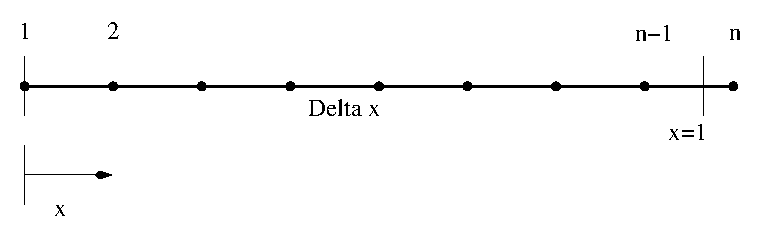
\epsfig{file=./Figures/oneddomain.eps, width=4in}\\
\caption{One dimensional domain in a grid mesh}\label{fig:onedomain}
\end{figurehere}
\end{center}
%
\vspace{2cm}
\begin{center}
\begin{figurehere}
\scalebox{0.8}{\input{./Figures/quadraticInterpolationf.pstex_t}}\\
\scalebox{0.8}{\input{./Figures/linearInterpolation.pstex_t}}\\
\caption{Top: linear Interpolation over partial element. Bottom: quadratic interpolation over full element adjacent to partial element}\label{fig:linear}
\end{figurehere}
\end{center}
\newpage
%
\begin{center}
\begin{figurehere}
\scalebox{1.0}{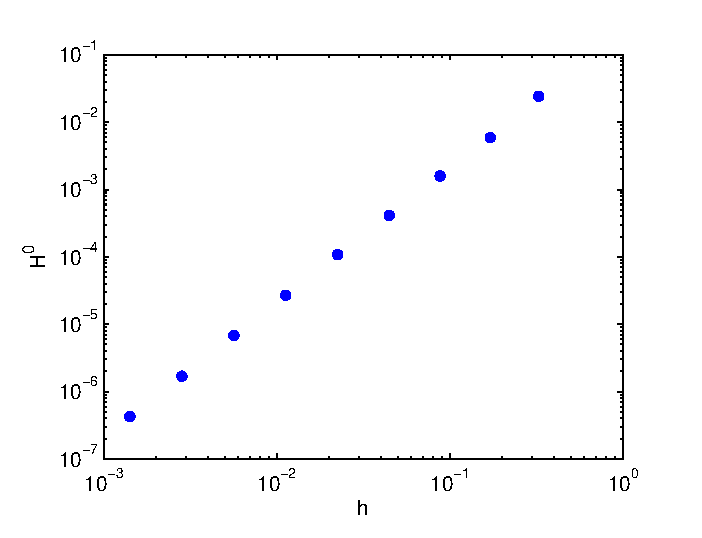
\includegraphics{./Figures/femdirichlet1dH0.eps}}\\
\scalebox{1.0}{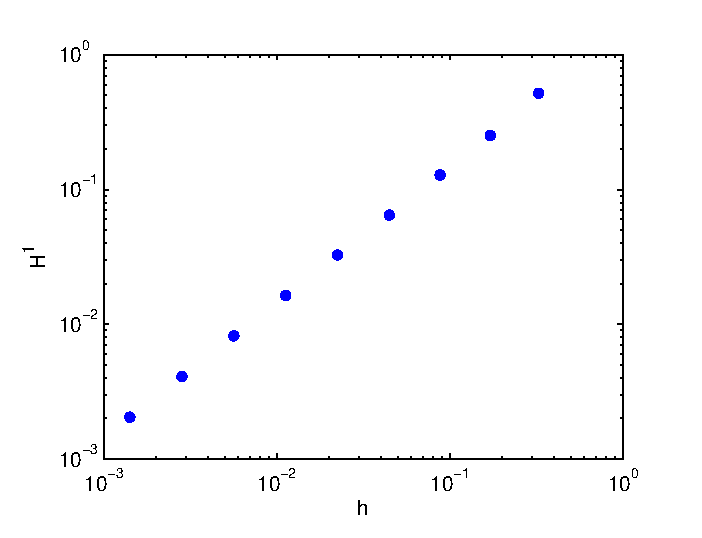
\includegraphics{./Figures/femdirichlet1dH1.eps}}\\
\caption{H$^0$- and H$^1$-convergence rate of one-dimensional Dirichlet-Dirichlet-problem solved with finite 
elements and partial cells}\label{fig:femdirichlet1dH0}
\end{figurehere}
\end{center}
\newpage
%
\begin{center}
\begin{figurehere}
\scalebox{1.0}{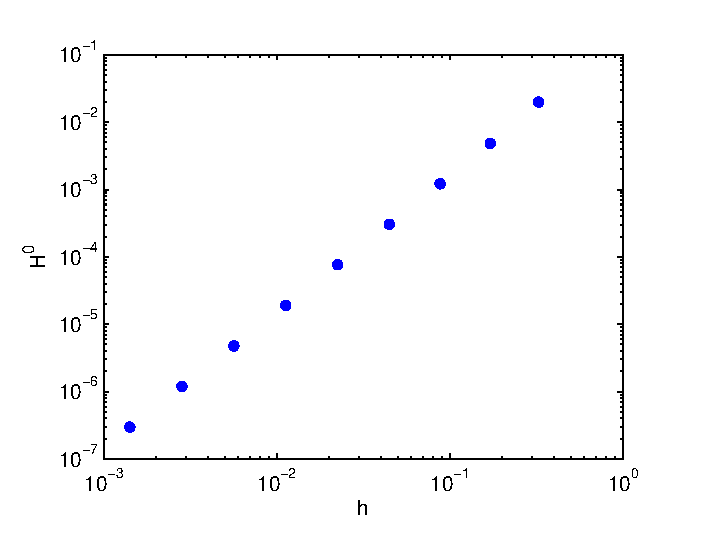
\includegraphics{./Figures/femneumann1dH0.eps}}\\
\scalebox{1.0}{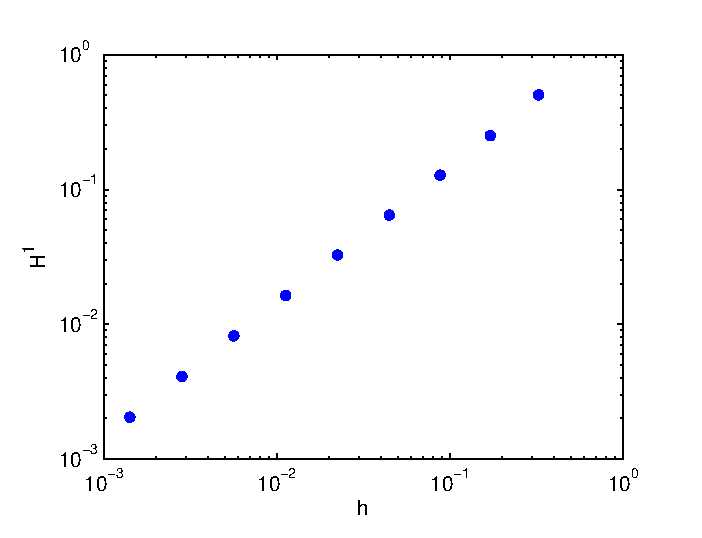
\includegraphics{./Figures/femneumann1dH1.eps}}\\
\caption{: H$^0$- and H$^1$-convergence rate of one-dimensional Dirichlet-Neumann-problem solved with finite elements and partial cells}\label{fig:femneumann1dH0}
\end{figurehere}
\end{center}
\newpage
%
\begin{center}
\begin{figurehere}
\scalebox{0.8}{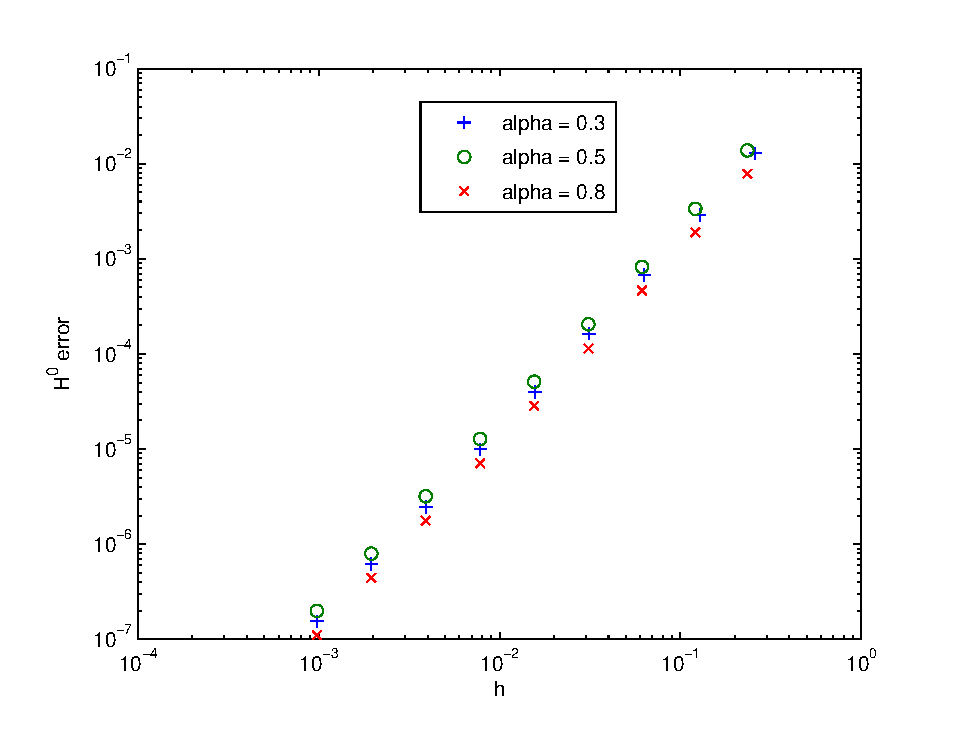
\includegraphics{./Figures/h0dirichlet.eps}}
\scalebox{0.8}{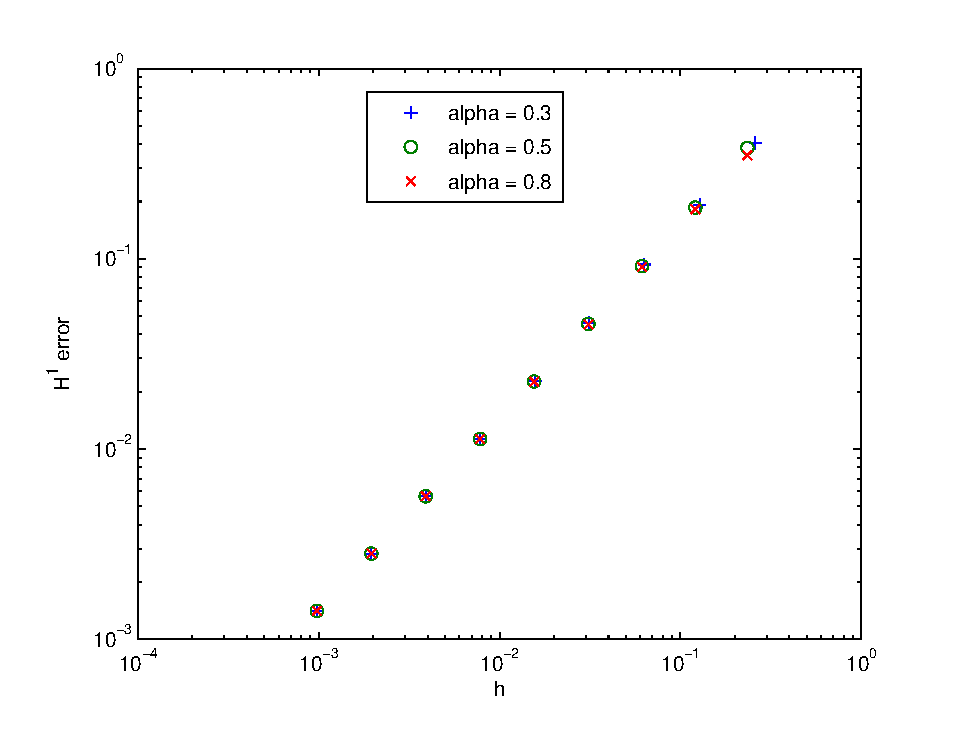
\includegraphics{./Figures/h1dirichlet.eps}}\\
\caption{Comparison of H$^0$- and H$^1$-convergence rates of a one-dimensional Dirichlet-Dirichlet-problem solved with finite elements and partial cells for different partial cells ratios $\alpha = 0.3, 0.5, 08$}\label{fig:dirichlet1dh0alpha030508}
\end{figurehere}
\end{center}
\newpage
%
\begin{center}
\begin{figurehere}
\scalebox{0.8}{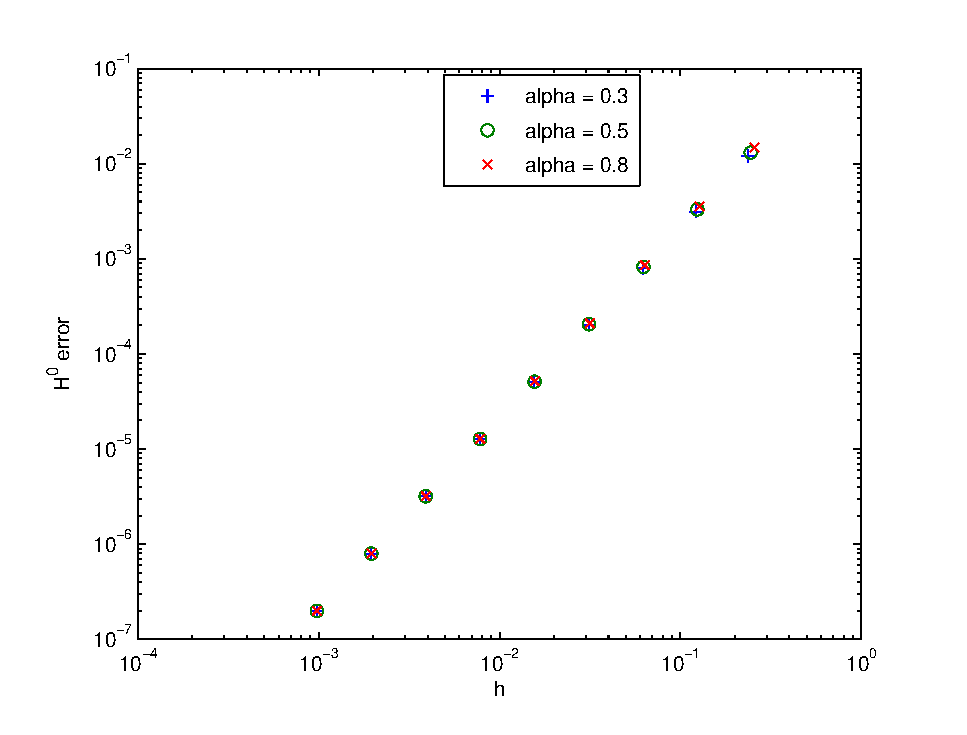
\includegraphics{./Figures/h0neumannlinear.eps}}\\
\scalebox{0.8}{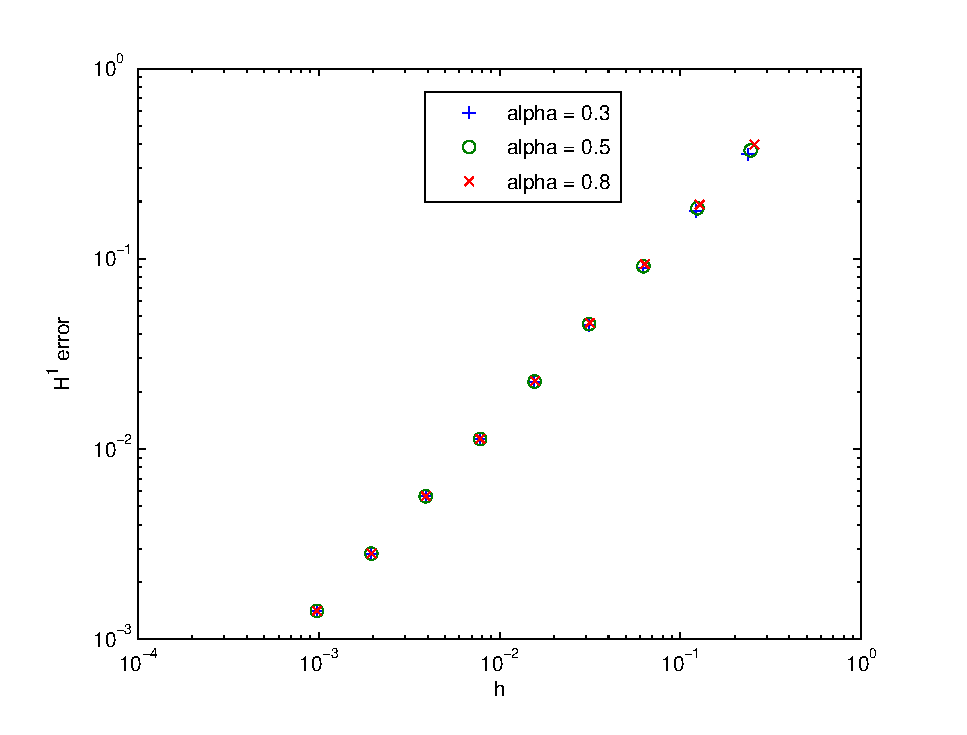
\includegraphics{./Figures/h1neumannlinear.eps}}\\
\caption{Comparison of H$^0$- and H$^1$-convergence rates of a one-dimensional Dirichlet-Neumann-problem solved with finite elements and partial cells for different partial cell ratios $\alpha = 0.3, 0.5, 08$}
\label{fig:neumann1dlinearh0alpha030508}
\end{figurehere}
\end{center}
\newpage
%
\begin{center}
\begin{figurehere}
\scalebox{0.8}{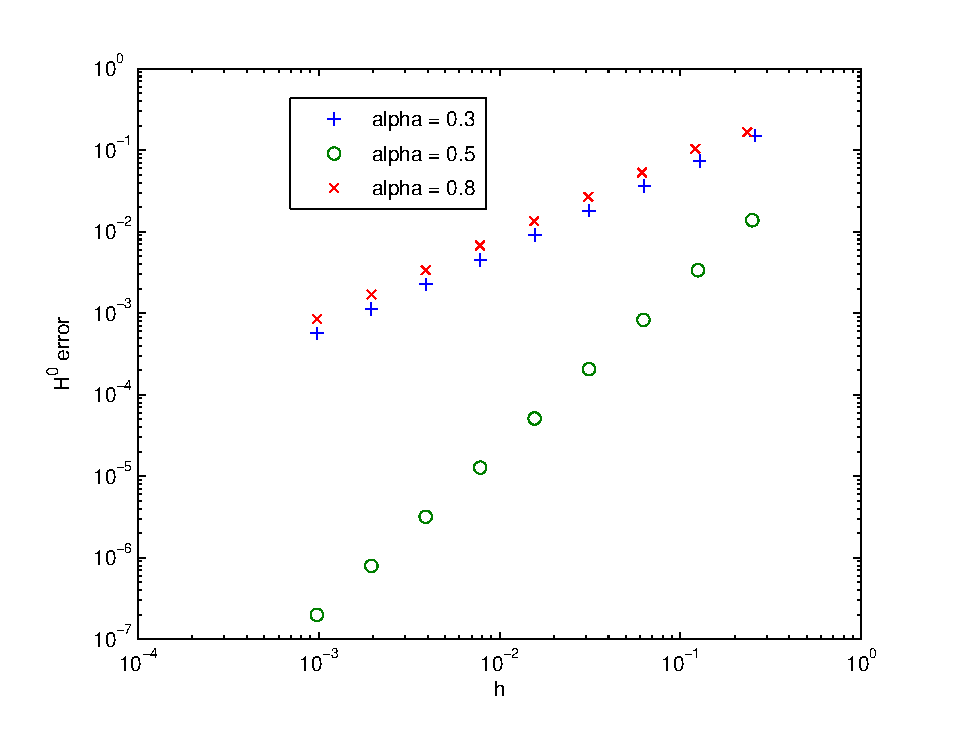
\includegraphics{./Figures/h0neumannconst.eps}}\\
\scalebox{0.8}{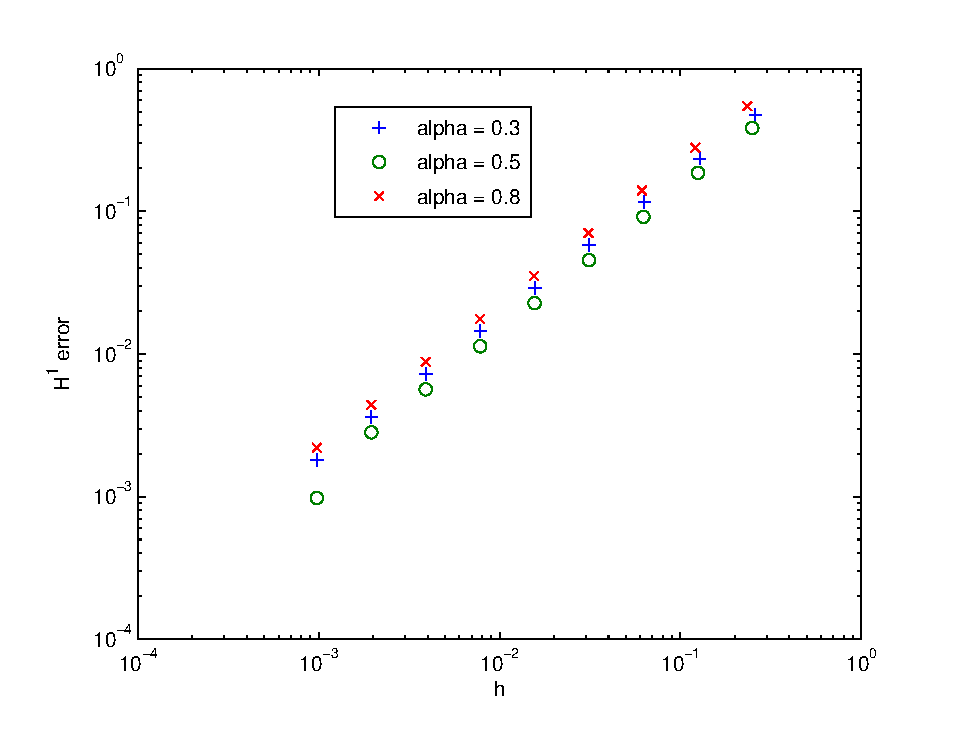
\includegraphics{./Figures/h1neumannconst.eps}}\\
\caption{Comparison of H$^0$- and H$^1$-convergences of  one-dimensional Dirichlet-Neumann-problem solved with finite Elements and partial Cells using constant interpolation of Neumann boundary condition for different partial cell ratios $\alpha = 0.3, 0.5, 0.8$}\label{fig:neumann1dconsth0alpha030508}
\end{figurehere}
\end{center}
\newpage
%
\begin{center}
\begin{figurehere} 
\scalebox{0.6}{\input{./Figures/partialelementcases.pstex_t}}\\
\caption{Partial Element Cases: (a) $3$ hanging nodes and $2$ intersection points (b) $2$ hanging nodes and $2$ intersection points (c) $1$ hanging node and $2$ intersection points}\label{fig:partialelements}
\end{figurehere}
\end{center}
\vspace{2cm}
%
\begin{center}
\begin{figurehere} 
\scalebox{0.7}{\input{./Figures/twoddomain.pstex_t}}\\
\caption{$3$ Types of elements: partial, full, void}\label{fig:elementtypes}
\end{figurehere}
\end{center}
\newpage
%
\begin{center}
\begin{figurehere} 
\scalebox{0.6}{\input{./Figures/specialpartialelements.pstex_t}}\\
\caption{Special cases of elements : (d) a void element, (e) an
interior element, (f) a partial element} 
\label{fig:specialcases}
\end{figurehere}
\end{center}
\vspace{2cm}
%
\begin{center}
\begin{figurehere} 
\scalebox{0.95}{\input{./Figures/interiorpoints.pstex_t}}\\
\caption{Calculation of intersection points for the cases: (a) one hanging node (b) two hanging nodes (c) three hanging nodes}
\label{fig:interiorpoints}
\end{figurehere}
\end{center}
\vspace{2cm}
%
\begin{center}
\begin{figurehere}
\input{./Figures/suspection.pstex_t}\\
\caption{Bad case for interpolating a Neumann boundary condition}\label{fig:suspection}
\end{figurehere}
\end{center}
\newpage
%
%\begin{center}
%\begin{figurehere} 
%\scalebox{0.7}{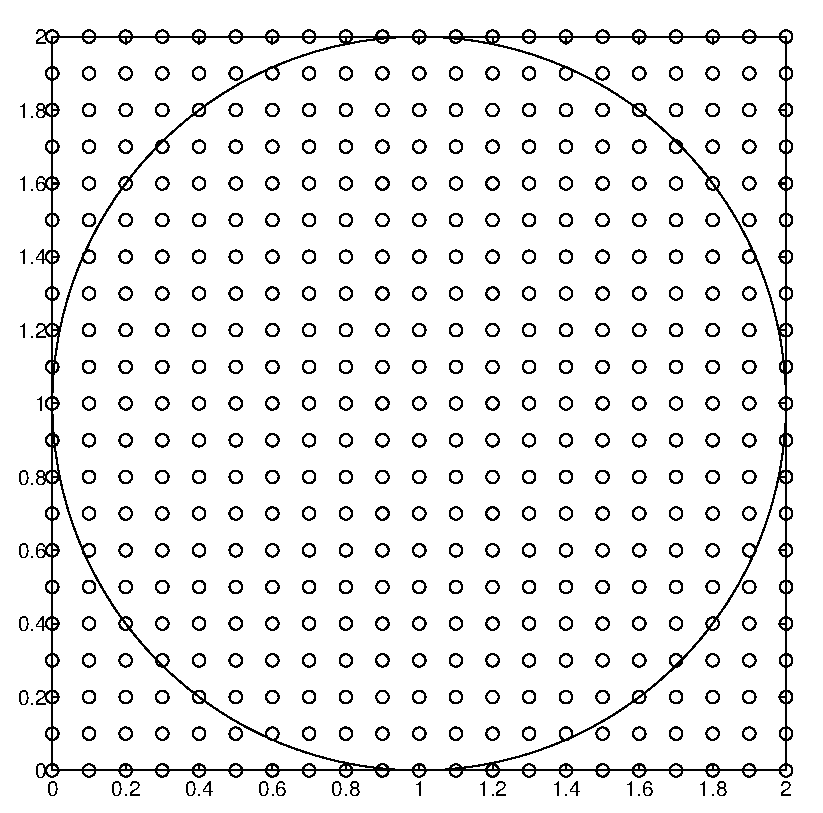
\includegraphics{./Figures/geometry.eps}}\\
%\caption{Circular Physical Domain and Cartesian Grid}\label{fig:geometry}
%\end{figurehere}
%\end{center}
%\newpage
%\clearpage
%
%\begin{center}
%\begin{figurehere}
%\scalebox{0.7}{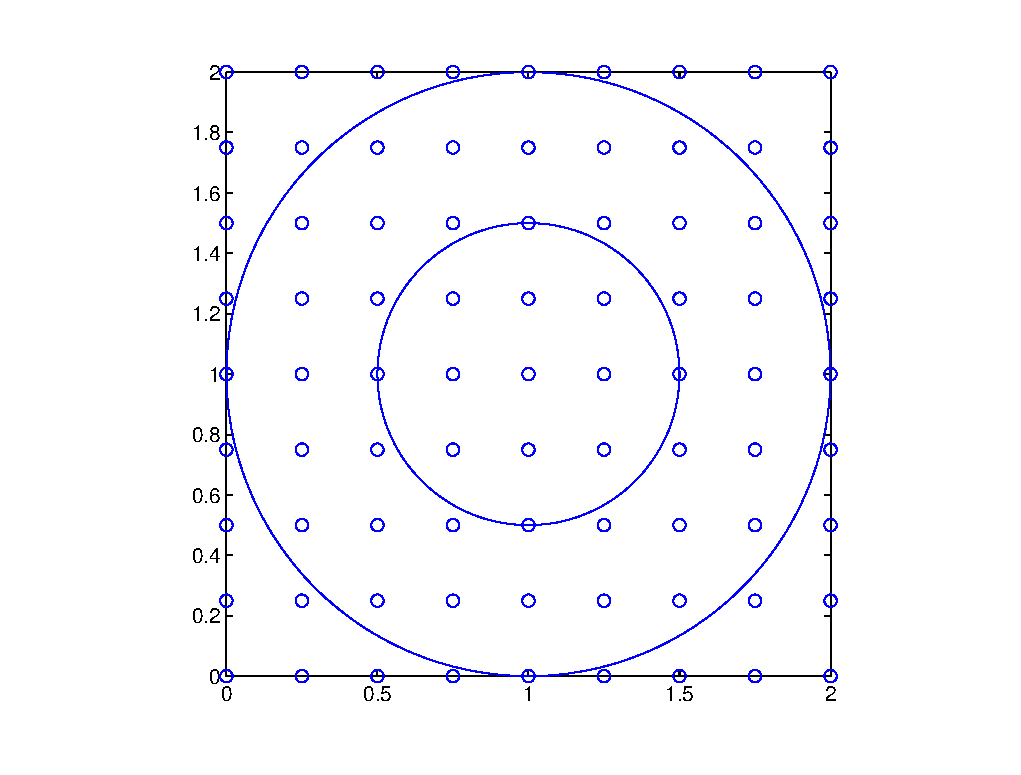
\includegraphics{./Figures/geomtorus.eps}}\\
%\caption{Annulus Geometry}\label{fig:torus}
%\end{figurehere}
%\end{center}
%\newpage
%
\begin{center}
\begin{figurehere}
\scalebox{0.7}{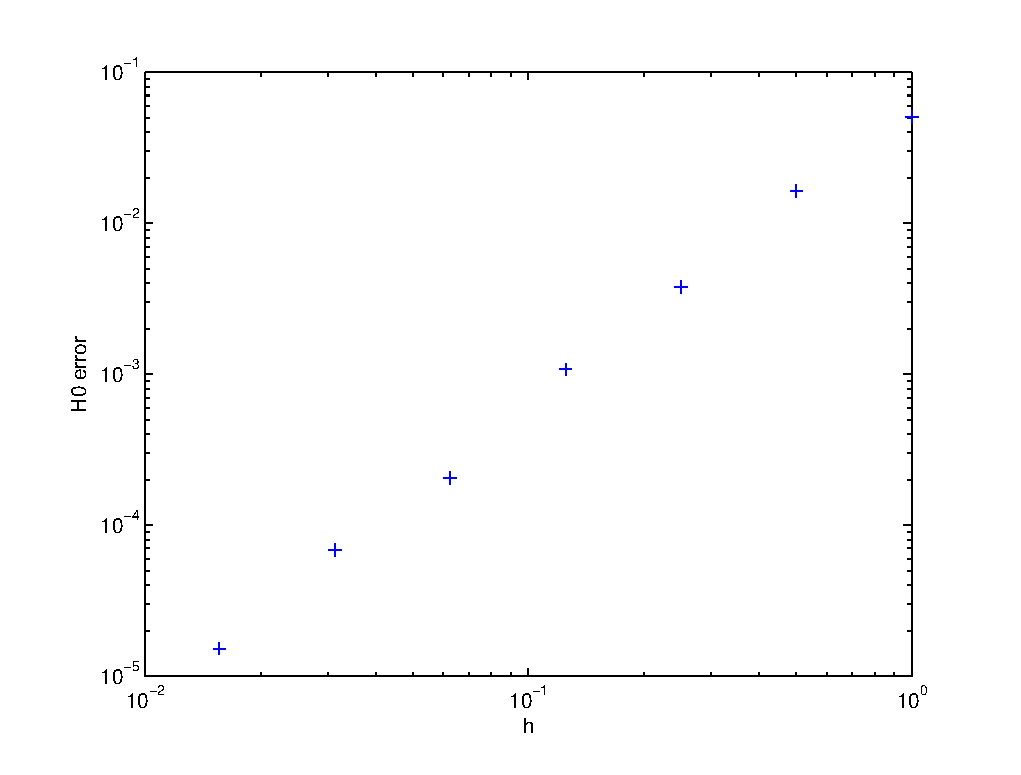
\includegraphics{./Figures/H0.eps}}\\
\scalebox{0.7}{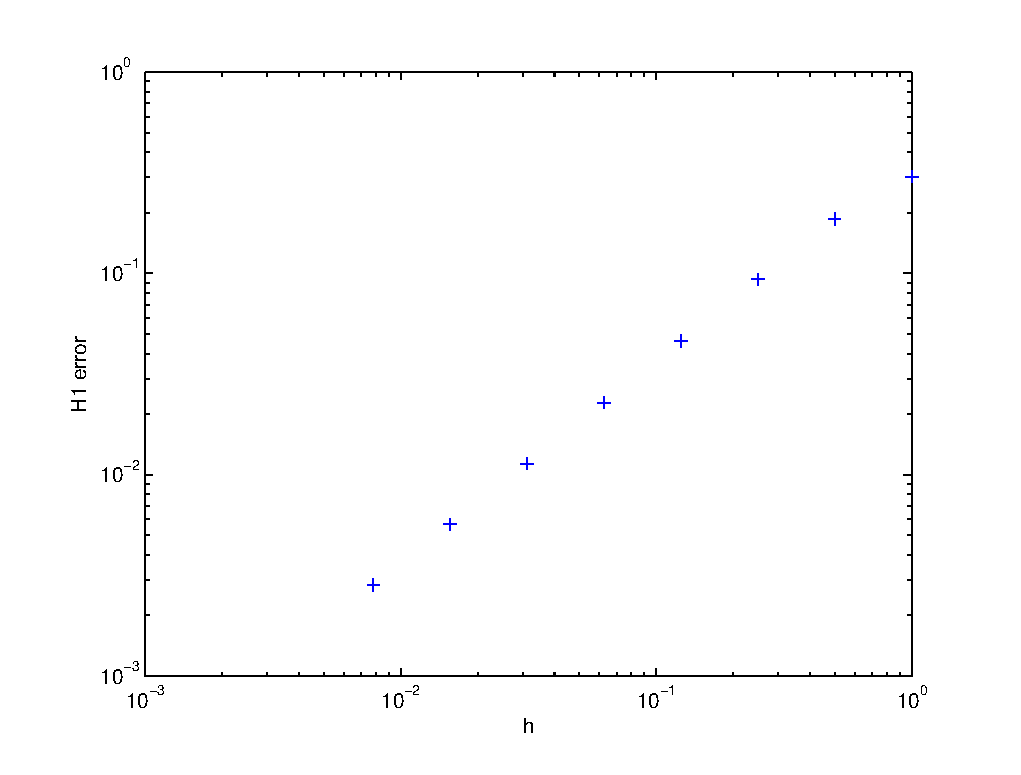
\includegraphics{./Figures/H1.eps}}\\
\caption{Convergence rate in the H$^0$- and  H$^1$-error norm of a Dirichlet Problem}\label{fig:H0new}
\end{figurehere}
\end{center}
\newpage
%
\begin{center}
\begin{figurehere}
\scalebox{0.7}{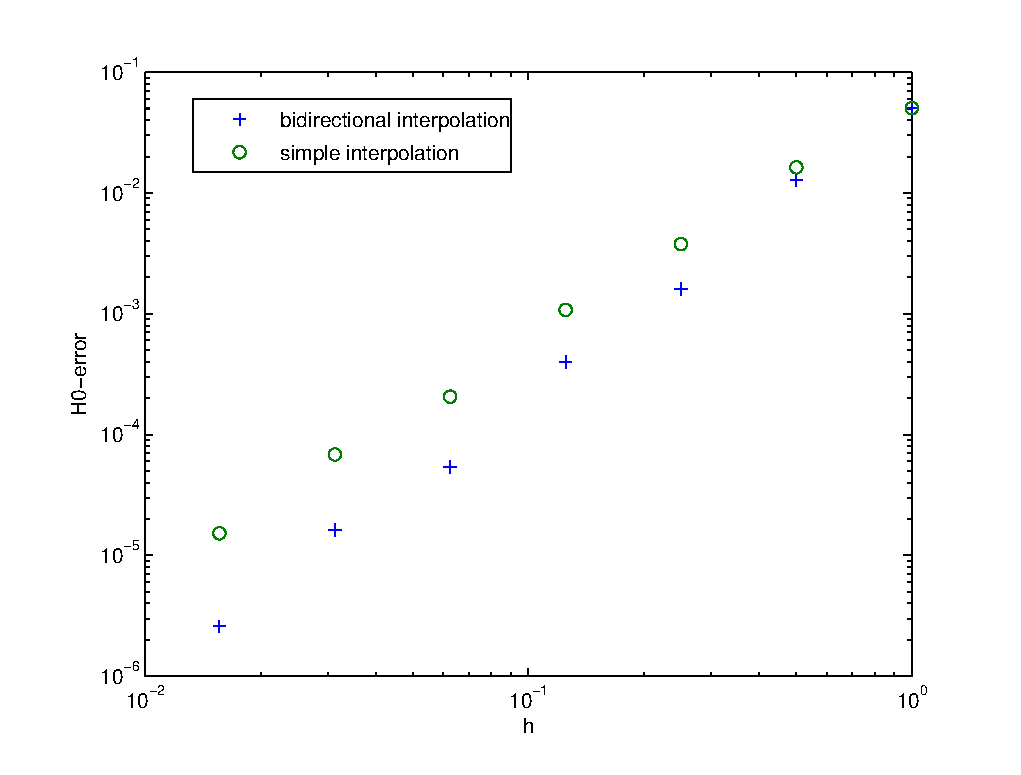
\includegraphics{./Figures/bidirecH0.eps}}\\
\scalebox{0.7}{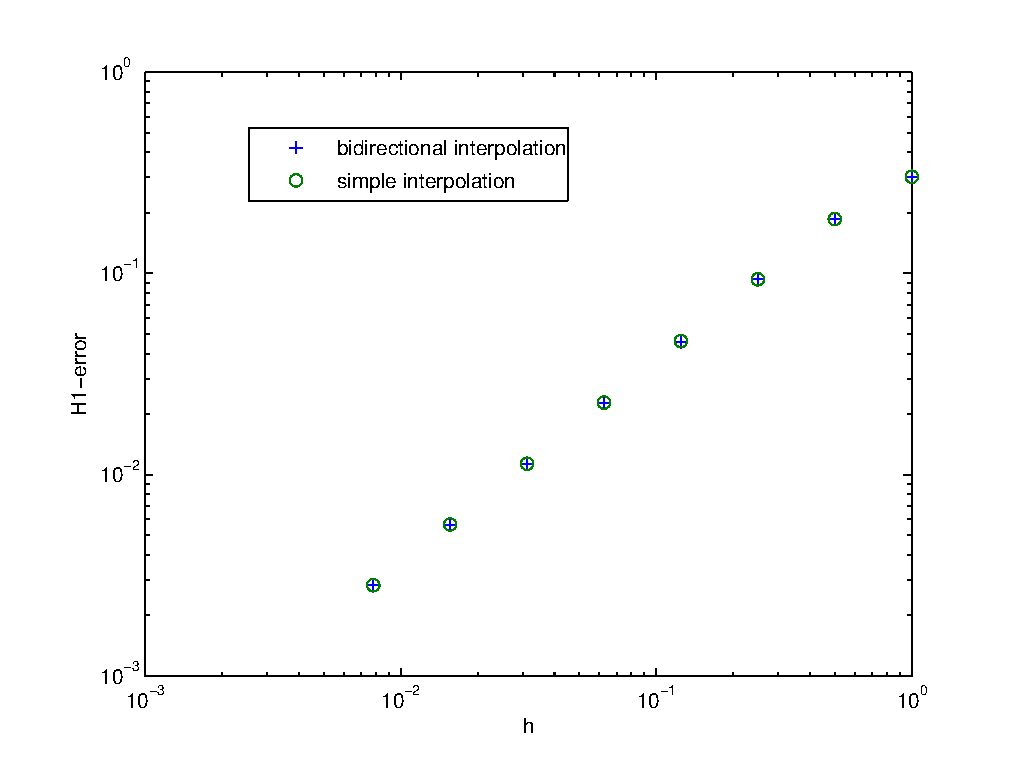
\includegraphics{./Figures/bidirecH1.eps}}\\
\caption{Convergence rate comparison of bi-directional and unidirectional interpolation in the H$^0$- and H$^1$-error norm}\label{fig:bidirecH0}
\end{figurehere}
\end{center}
\newpage
%
\begin{center}
\begin{figurehere}
\scalebox{0.7}{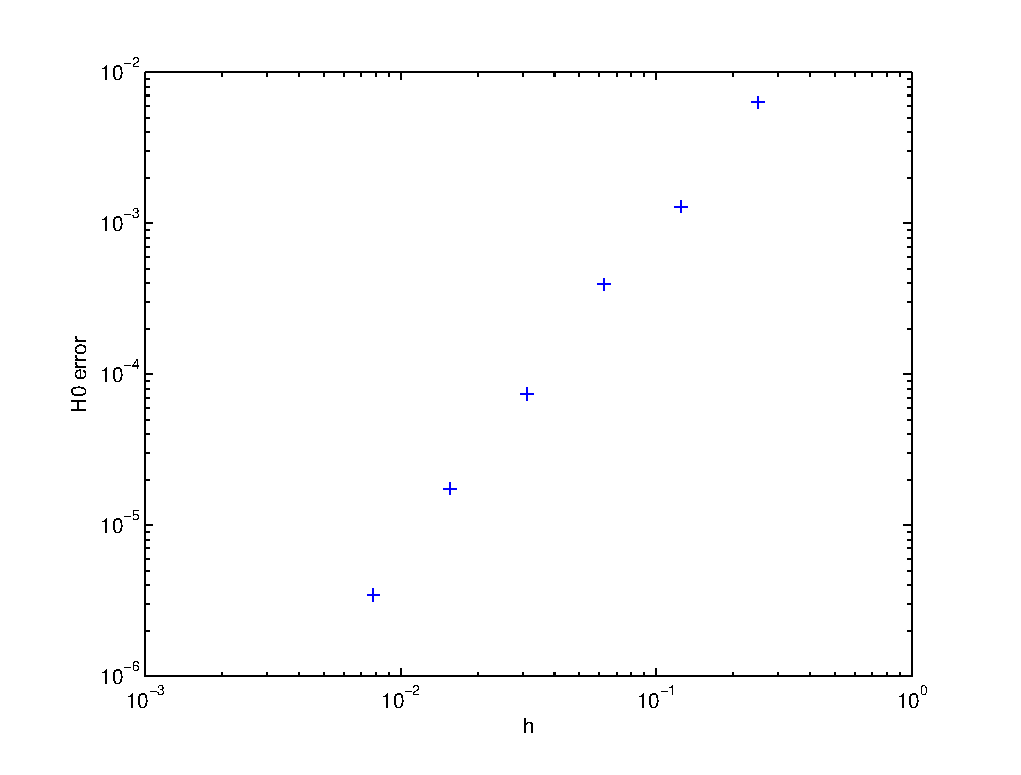
\includegraphics{./Figures/h0errtorus.eps}}\\
\scalebox{0.7}{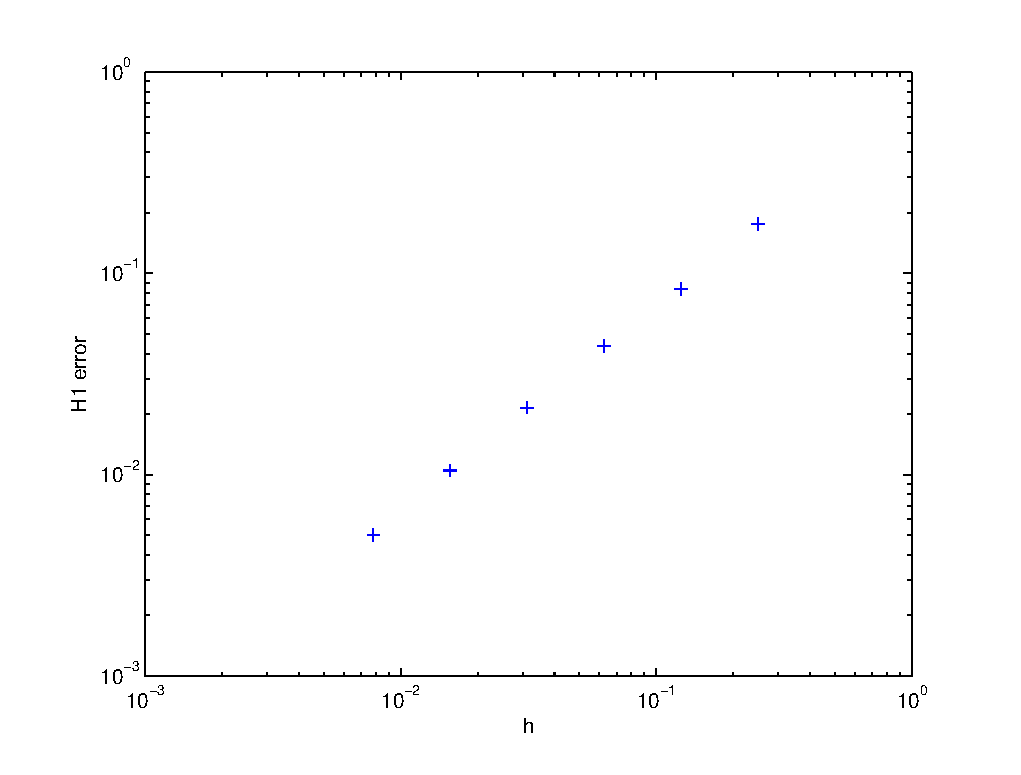
\includegraphics{./Figures/h1errtorus.eps}}\\
\caption{Convergence rate in the H$^0$- and H$^1$-error norm of an annular domain with Dirichlet-Dirichlet boundary conditions}\label{fig:h0torus}
\end{figurehere}
\end{center}
\newpage
%
\begin{center}
\begin{figurehere}
\scalebox{0.7}{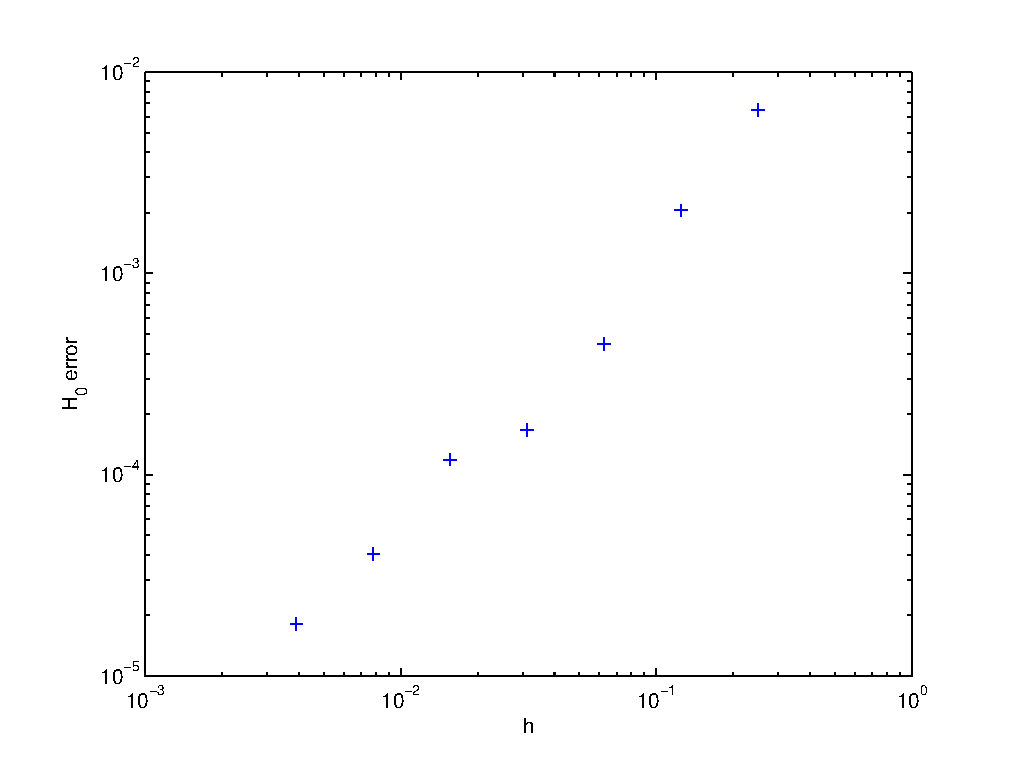
\includegraphics{./Figures/convergenceH0torus.eps}}\\
\scalebox{0.7}{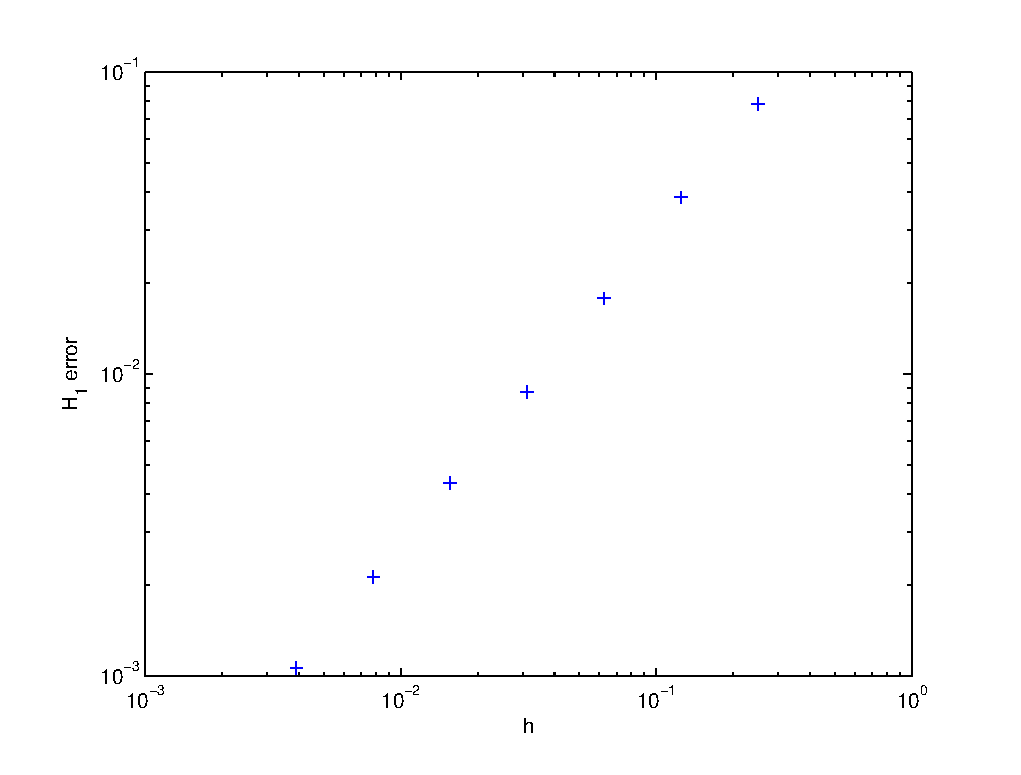
\includegraphics{./Figures/convergenceH1torus.eps}}\\
\caption{Convergence rate in the H$^0$- and H$^1$error norm}\label{fig:convergencetorusH0}
\end{figurehere}
\end{center}
\newpage
%
%\begin{center}
%\begin{figurehere}
%\scalebox{0.9}{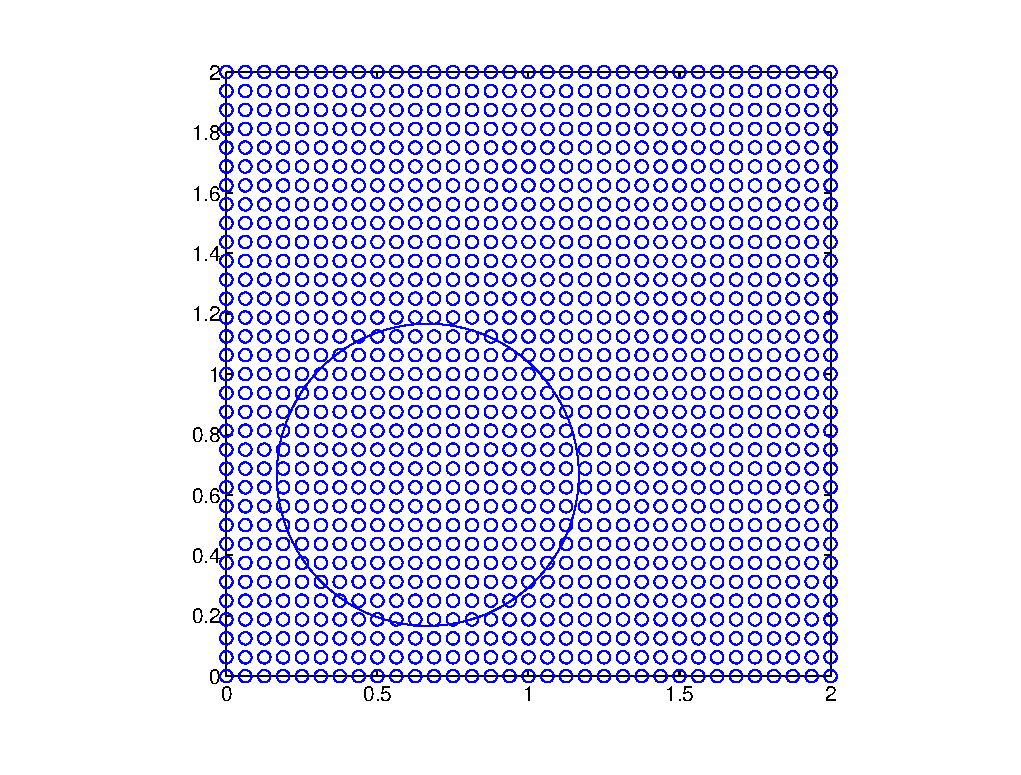
\includegraphics{./Figures/shiftedcircle.eps}}
%\caption{Shifted circle with respect to the grid center}\label{fig:shiftedcircle}
%\end{figurehere}
%\end{center}
%\newpage
%
\begin{center}
\begin{figurehere}
\scalebox{1.0}{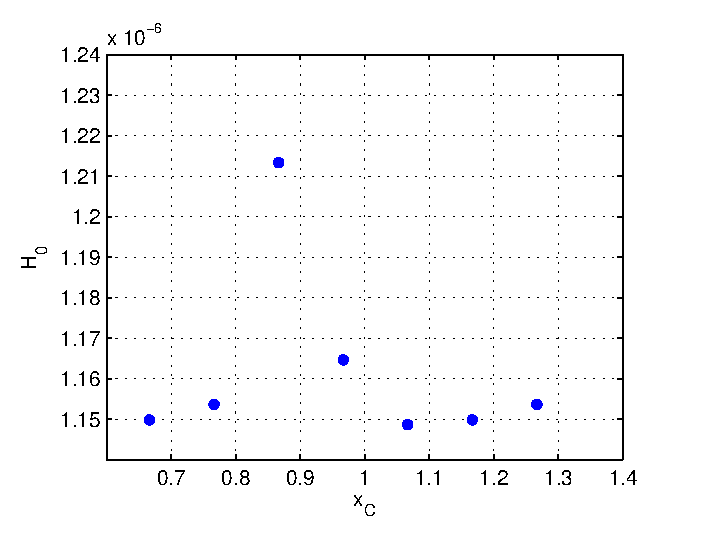
\includegraphics{./Figures/dirichletcircleh0x.eps}}\\
\scalebox{1.0}{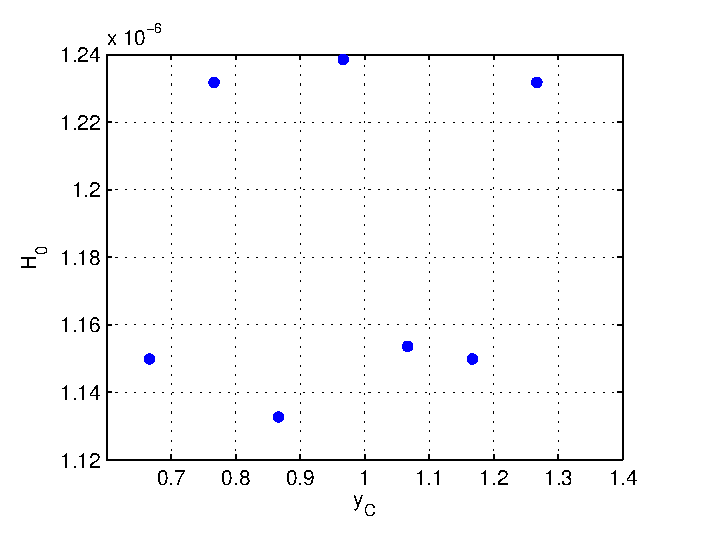
\includegraphics{./Figures/dirichletcircleh0y.eps}}\\
\caption{H$^0$-convergence rate of shifting the Dirichlet circle center along x-direction and y-direction}\label{fig:shiftcircledirichletH0xy}
\end{figurehere}
\end{center}
\newpage
%
\begin{center}
\begin{figurehere}
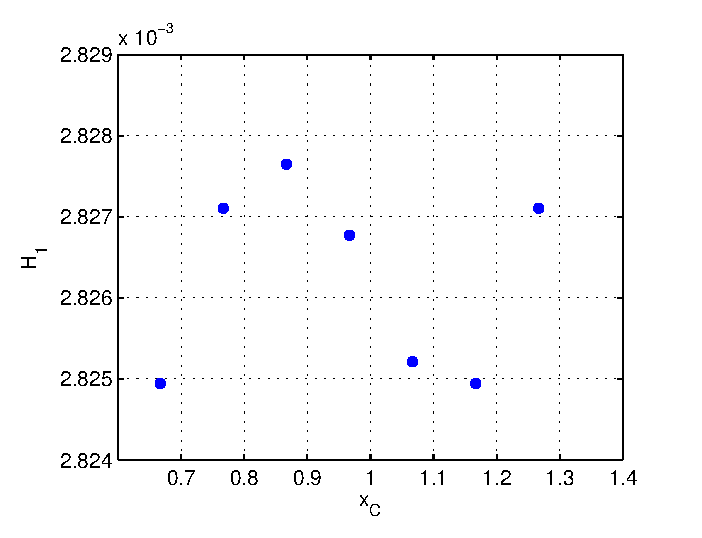
\includegraphics[scale=1.0]{./Figures/dirichletcircleh1x.eps}\\
\scalebox{1.0}{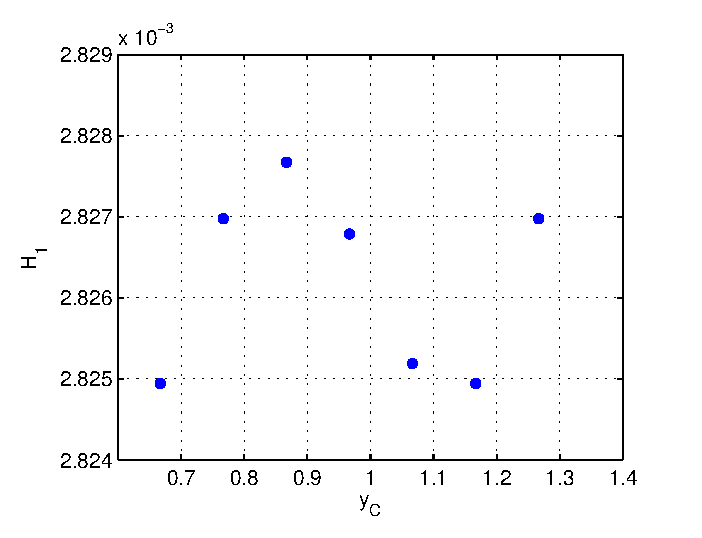
\includegraphics{./Figures/dirichletcircleh1y.eps}}\\
\caption{H$^1$-convergence rate of shifting the Dirichlet circle center along x-direction and y-direction}\label{fig:shiftcircledirichletH1xy}
\end{figurehere}
\end{center}
\newpage
%
\begin{center}
\begin{figurehere}
\scalebox{1.0}{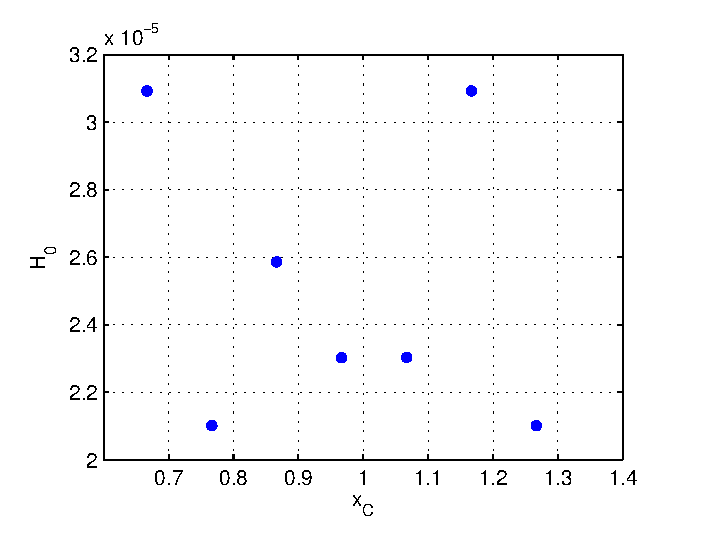
\includegraphics{./Figures/dirichlettorush0x.eps}}\\
\scalebox{1.0}{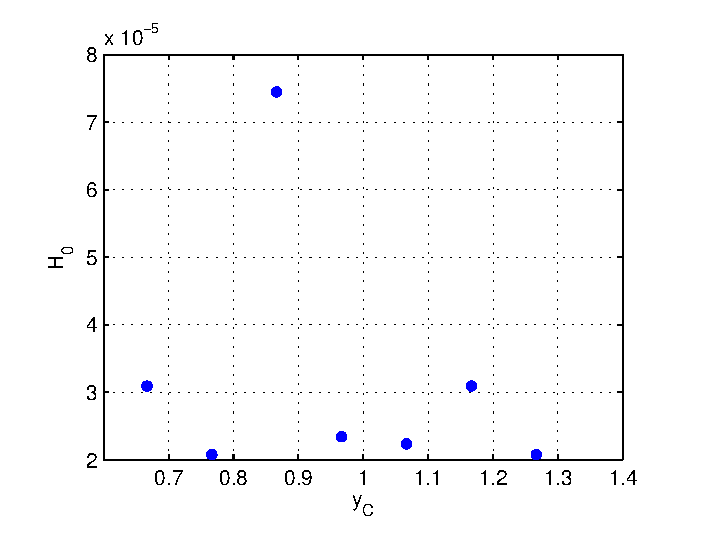
\includegraphics{./Figures/dirichlettorush0y.eps}}\\
\caption{ H$^0$-convergence rate of shifting the Dirichlet annulus center along x-direction and y-direction}\label{fig:shifttorusdirichletH0xy}
\end{figurehere}
\end{center}
\newpage
%
\begin{center}
\begin{figurehere}
\scalebox{1.0}{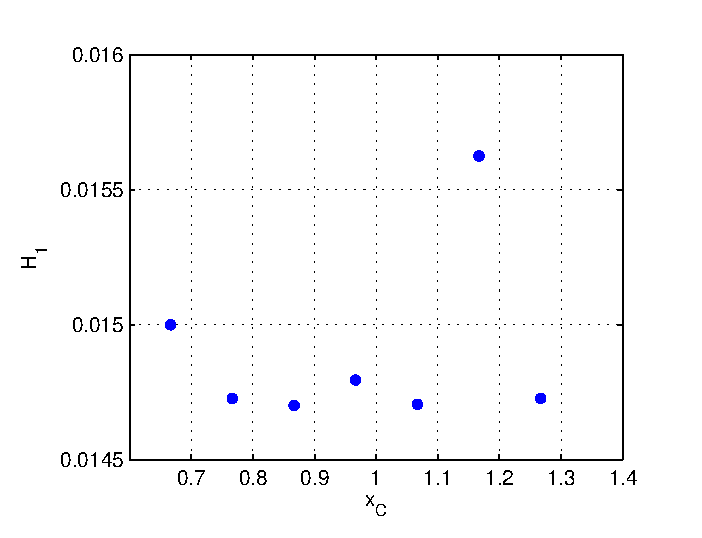
\includegraphics{./Figures/dirichlettorush1x.eps}}\\
\scalebox{1.0}{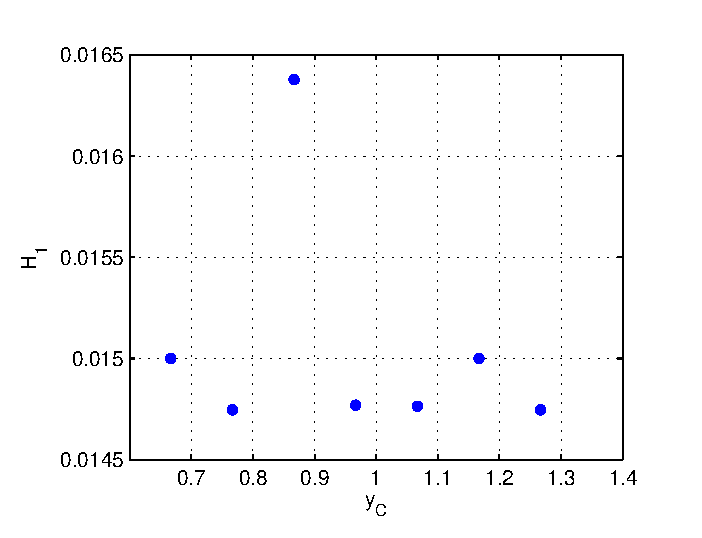
\includegraphics{./Figures/dirichlettorush1y.eps}}\\
\caption{H$^1$-convergence rate of shifting the Dirichlet annulus center along x-direction and y-direction:  }\label{fig:shifttorusdirichletH1xy}
\end{figurehere}
\end{center}
\newpage
%
\begin{center}
\begin{figurehere}
\scalebox{1.0}{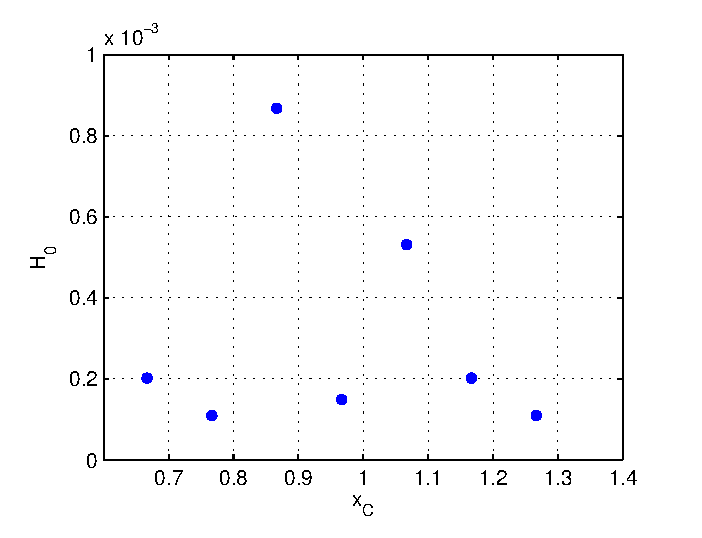
\includegraphics{./Figures/neumanntorush0x.eps}}\\
\scalebox{1.0}{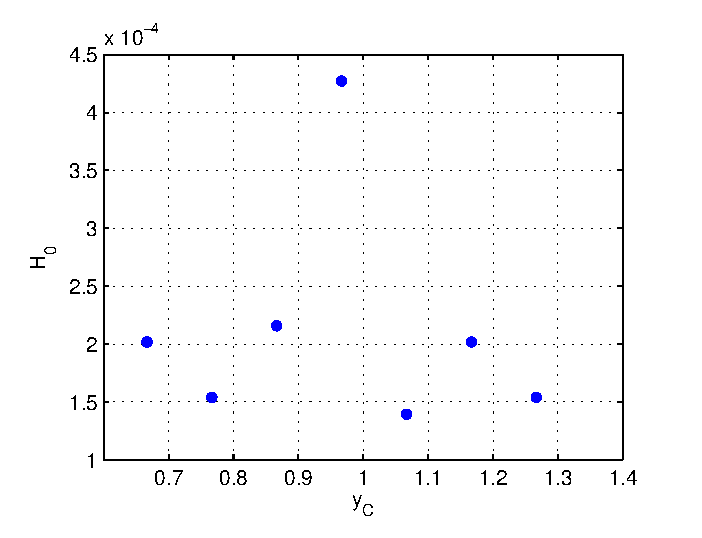
\includegraphics{./Figures/neumanntorush0y.eps}}\\
\caption{H$^0$-convergence rate of shifting the Neumann-Dirichlet annulus center along x-direction and y-direction}\label{fig:shifttorusneumannH0xy}
\end{figurehere}
\end{center}
\newpage
%
\begin{center}
\begin{figurehere}
\scalebox{1.0}{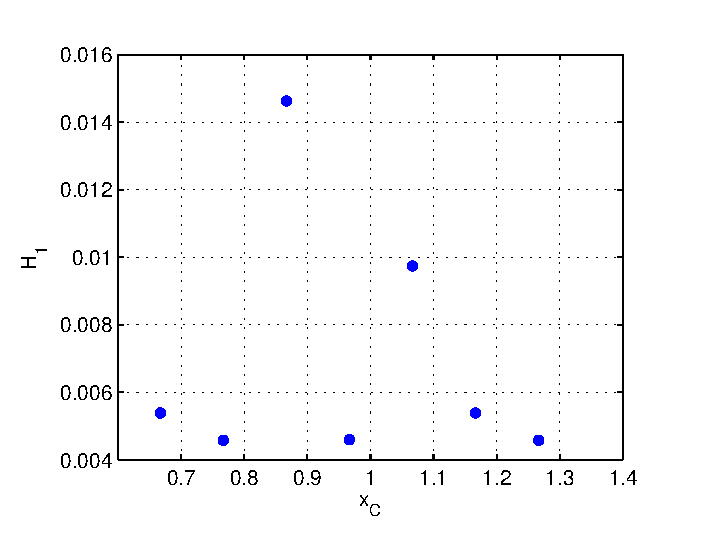
\includegraphics{./Figures/neumanntorush1x.eps}}\\
\scalebox{1.0}{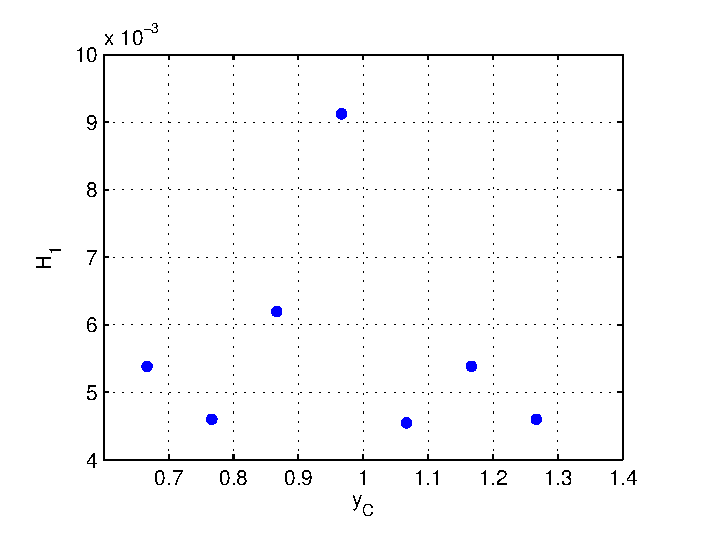
\includegraphics{./Figures/neumanntorush1y.eps}}\\
\caption{H$^1$-convergence rate of shifting the Neumann-Dirichlet annulus center along x-direction and y-direction}\label{fig:shifttorusneumannH1xy}
\end{figurehere}
\end{center}
\newpage
%
\begin{center}
\begin{figurehere}
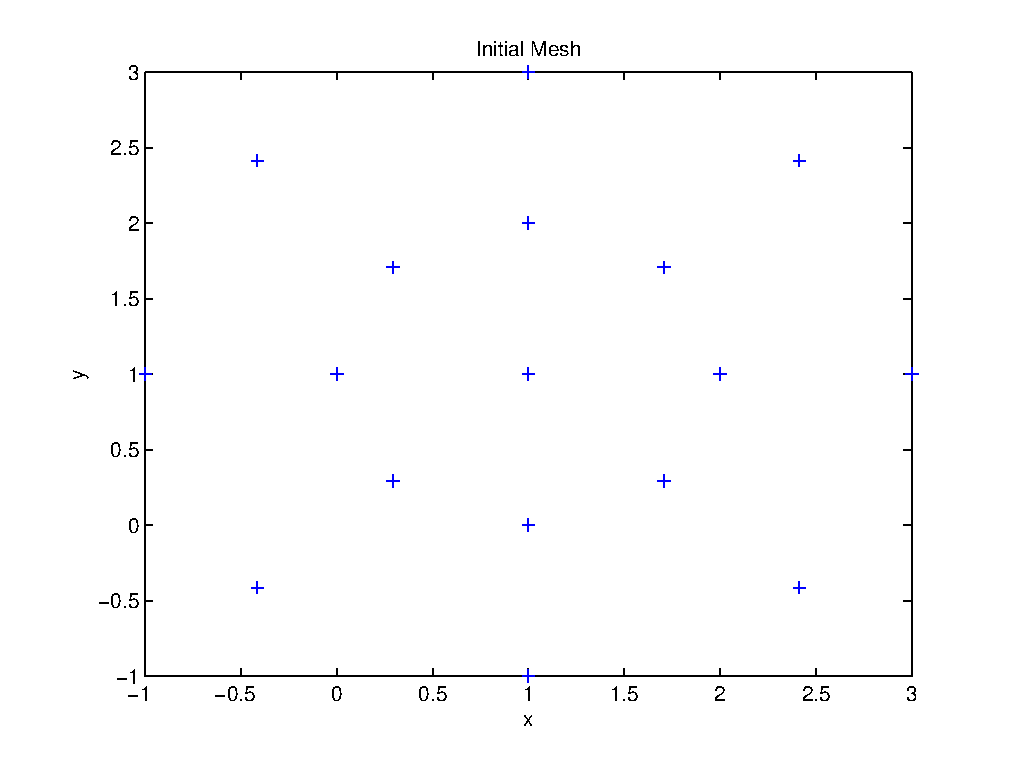
\includegraphics[width=49mm, height=49mm]{./Figures/initial.eps}
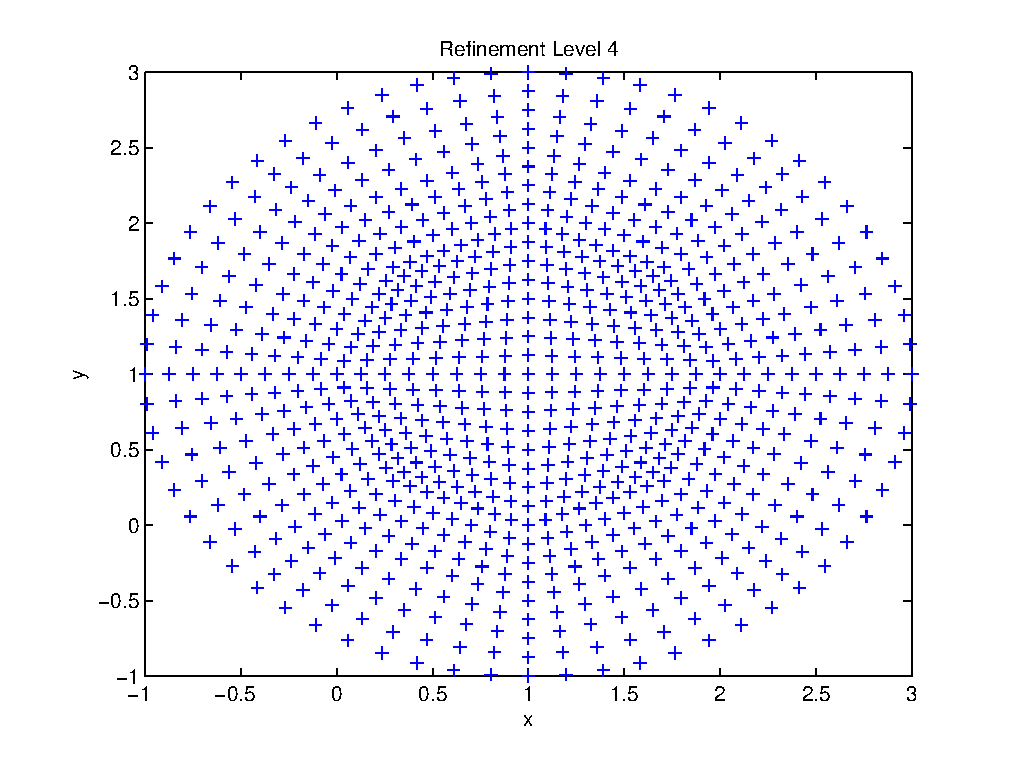
\includegraphics[width=49mm, height=49mm]{./Figures/level4.eps}
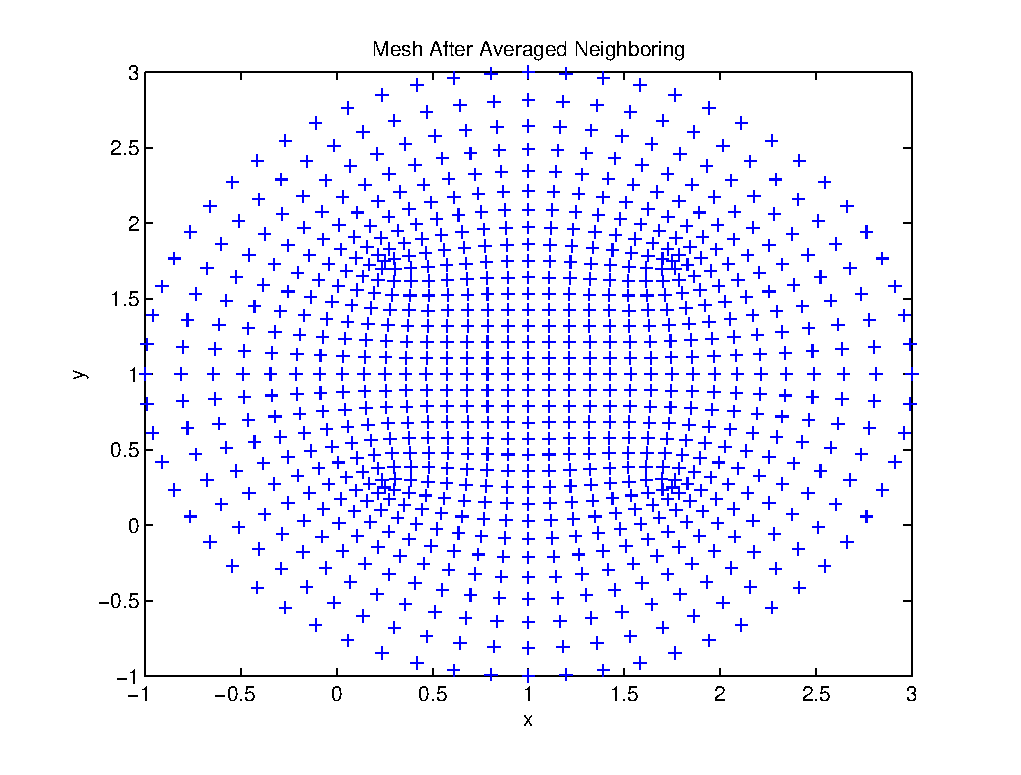
\includegraphics[width=49mm, height=49mm]{./Figures/level4avg.eps}\\
\caption{Initial Mesh, finer Mesh, neighbor Averaged Mesh}\label{fig:refine}
\end{figurehere}
\end{center}
\newpage

%
\begin{center}
\begin{figurehere}
\scalebox{0.7}{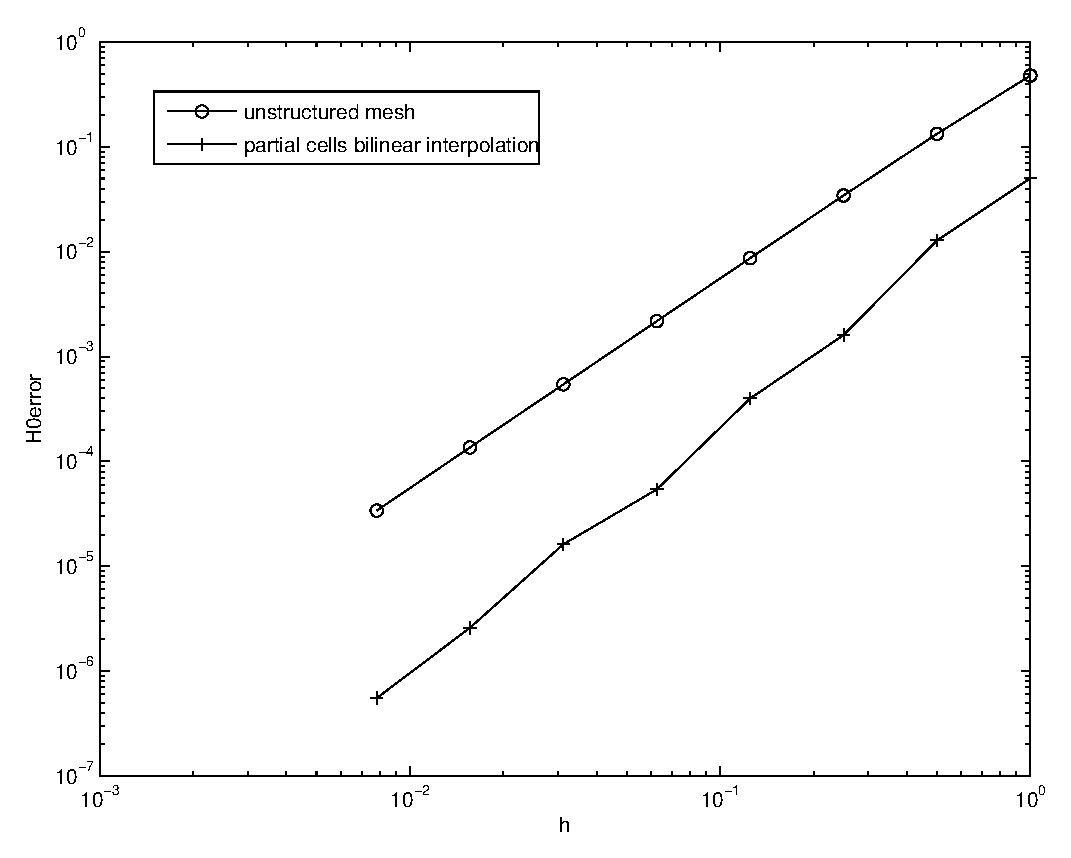
\includegraphics{./Figures/comparstrucunstrH0.eps}}\\
\scalebox{0.7}{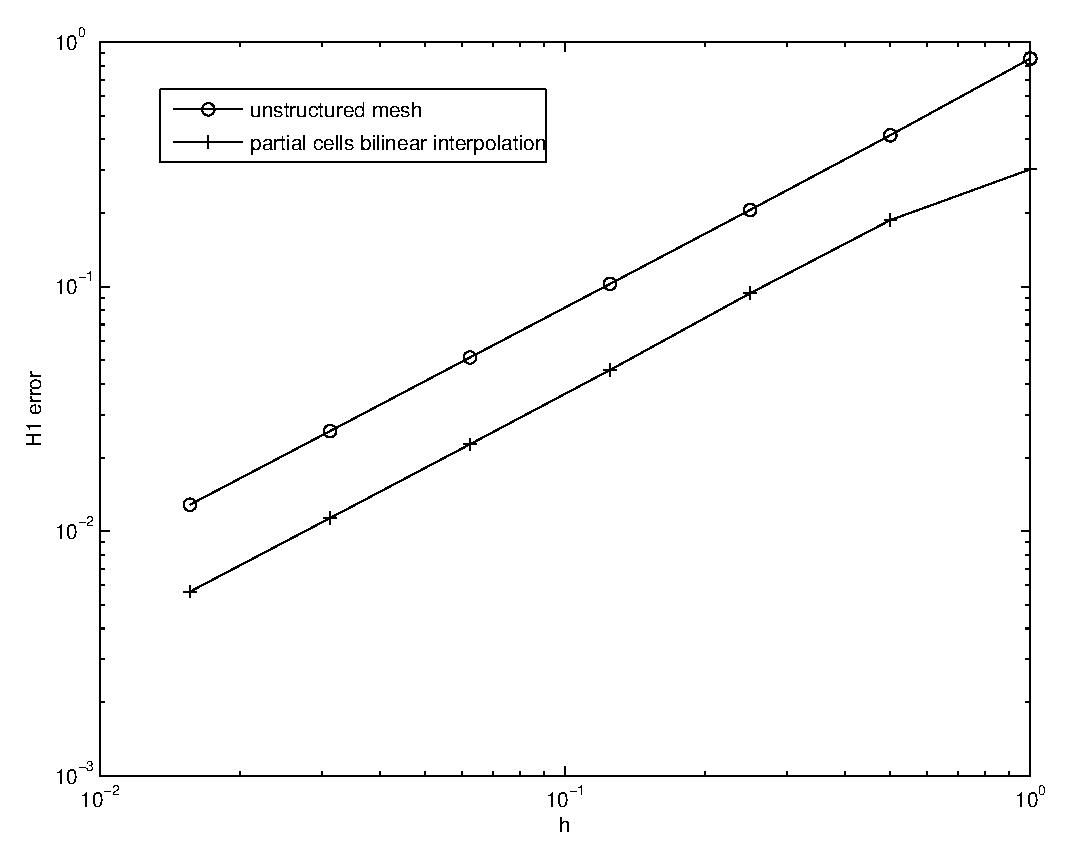
\includegraphics{./Figures/comparstrucunstrH1.eps}}\\
\caption{Convergence rate comparison of structured vs. unstructured mesh in the H$^0$- and H$^1$-error norm}\label{fig:comparH0}
\end{figurehere}
\end{center}
\newpage
%
\begin{center}
\begin{figurehere}
\scalebox{0.7}{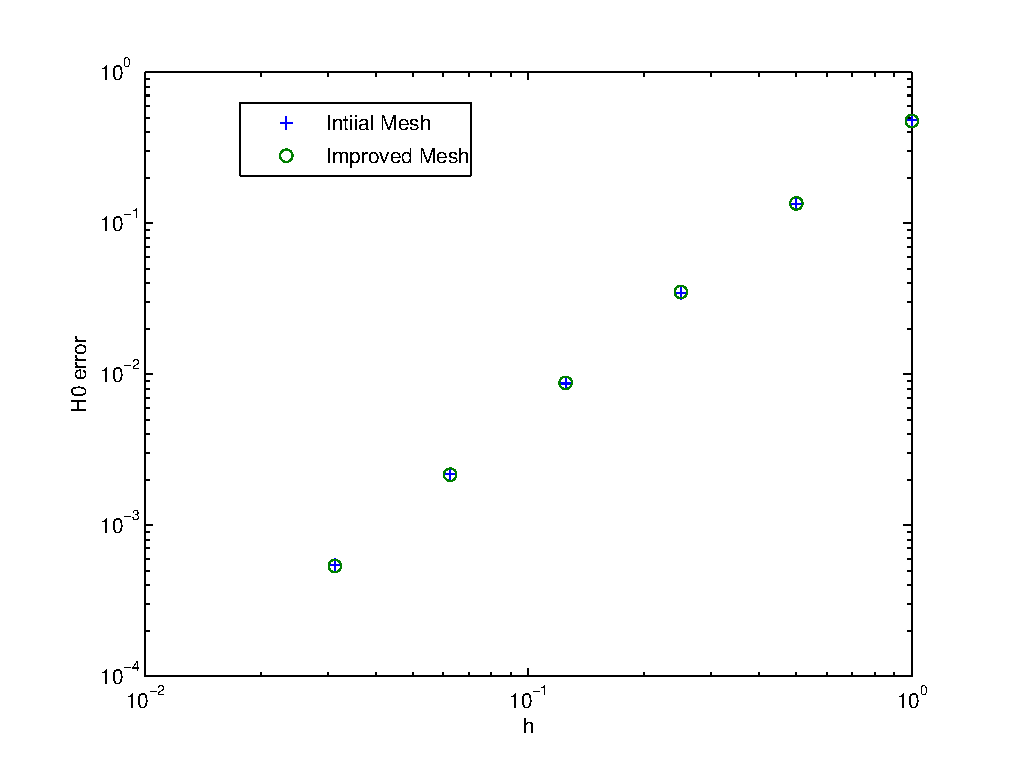
\includegraphics{./Figures/comparH0impr.eps}}\\
\scalebox{0.7}{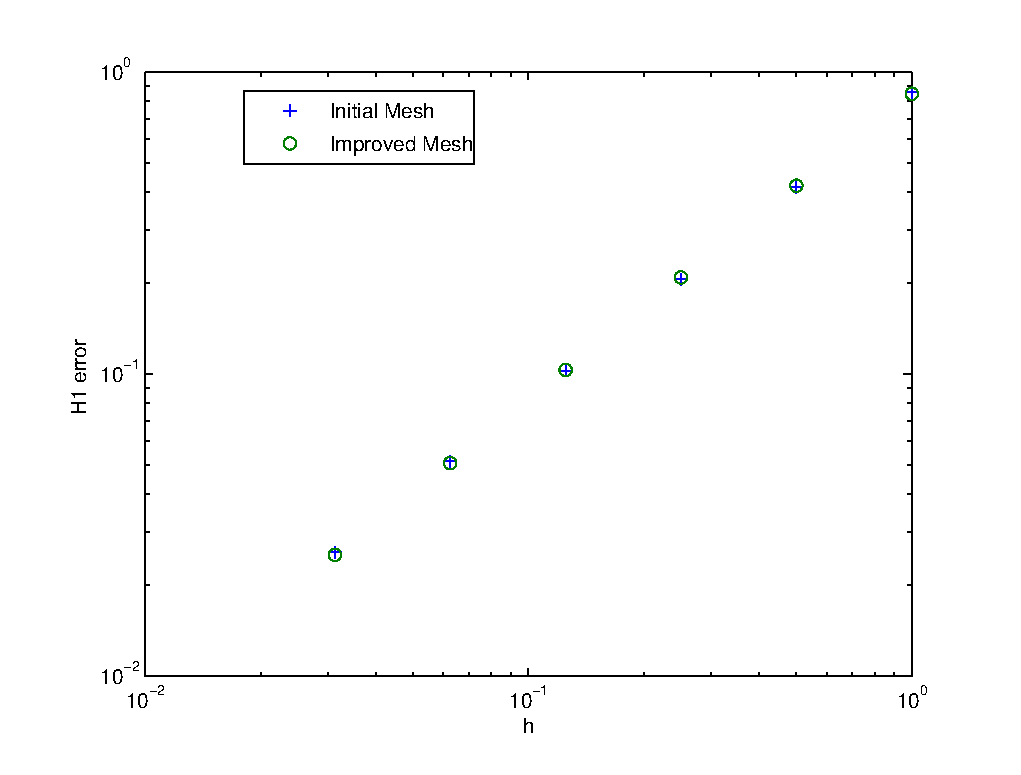
\includegraphics{./Figures/comparH1impr.eps}}\\
\caption{Convergence rate comparison of initial vs. improved mesh in the H$^0$- and H$^1$-error norm}\label{fig:comparH0impr}
\end{figurehere}
\end{center}
\newpage
%
%
%********************************BOX-ALGORITHM**********************************
%

\section{Algorithm}
%\clearpage
\begin{algorithm}
%\dontprintsemicolon
\Begin{
Generate a bounding box surrounding the physical domain\;
Generate a uniform regular grid bounded by the bounding box\;
\For{elements}{
\If{full element}{set flag to 1\;}
\ElseIf{partial element}{set flag to 2\;}
\Else{{\em  void element, set flag to 3\;}}
%
\If{flag = 1 $\Vert$ flag = 2}{
Calculate finite element arrays for whole element
}
\If{flag = 2}{
Identify hanging nodes H (and degrees of freedom) of element, and 
intersection points N of element edges with physical boundary\; 
%
Determine nature of boundary condition (Dirichlet or Neumann) 
for physical boundary traversing the element\; 
%
\If{Neumann boundary condition}{
\If{H = 1 \& hanging node is intersection point}{set flag to 1\;
\Return}
}
\If{bi-directional interpolation}{
Create new intersection points NI on physical boundary traversing
the element and set N=NI\;
}
\If{H $>$ N}{
Generate additional interpolation points on the physical boundary 
traversing the element\;
}
Determine pairing of hanging nodes to intersection/sampling points\;
}
}
Assemble element arrays\;
\For{elements}{
\If{flag = 2}{
\For{hanging node-to-intersection/sampling points}{ 
Set all coefficients corresponding to hanging node degrees of freedom
to zero in global equations\;
}
\For{hanging node-to-intersection/sampling points}{ 
Assemble into global system all equations generated from enforcement
of boundary conditions for hanging node degrees of freedom\;
}
}
}
Solve the algebraic system\;
}
\caption{Algorithm for cut-cells in structured finite elements}
\end{algorithm}


\end{document}
